 % Vorspann
% ----------------------------------------------
	\documentclass[12pt,a4paper,bibtotoc, liststotoc, headsepline]{scrreprt}

%\documentclass[
%a4paper,
%12pt,
%oneside,
%headings=big,
%chapterprefix,
%headsepline
%]{scrbook}
%\usepackage[T1]{fontenc} % Ausgabe-Encoding
%\usepackage[utf8]{inputenc}% Eingabe-Encoding
%\usepackage[ngerman]{babel}% deutsch
%\usepackage{scrpage2} % Kopf und Fu�
%
%\pagestyle{scrheadings}
%\setkomafont{pageheadfoot}{\normalfont\bfseries}
%\renewcommand*\chapterpagestyle{scrheadings}
%\renewcommand*\sectionmark[1]{\markright{\thesection\ #1}} 
%
%% Kopf
%\ihead{} % innen oder links
%\chead{}
%\ohead{\headmark} % au�en oder rechts
%
%% Fu�
%\ifoot{} % innen oder lnks
%\cfoot{}
%\ofoot{\pagemark} % au�en oder rechts



%\documentclass{scrreprt}
%\usepackage{blindtext}
%\usepackage[automark]{scrlayer-scrpage}
%\pagestyle{scrheadings}
%\ifoot[\TeX nische Universit\"at]{\TeX nische Universit\"at}
%%\chead[\headmark]{\headmark}
%\begin{document}
%\blinddocument
%
%\pagestyle{plain}
%%Von nun an nur noch im style plain
%\blinddocument
%
%\pagestyle{empty}
%\chapter{Und nun empty}
%%Die erste Seite wird nat�rlich noch im Stil plain gesetzt.
%%Also legen wir direkt nach chapter den Seitenstil lokal fest. 
%\thispagestyle{empty}
%\blindtext[6]
%\end{document}
%\documentclass[ 
%12pt, 
%a4paper, 
%headinclude, 
%footinclude, 
%plainfootsepline]{scrreprt} 
%\usepackage{scrpage2} 
%
%\pagestyle{scrheadings} 
%\clearscrheadfoot 
%\automark{chapter} 
%   \ihead{\headmark}   
%   \cfoot[-{ }\pagemark{ }-]{-{ }\pagemark{ }-} 
%%Bei der Einstellung der Seitenstile bietet KOMA-Script direkt die M�glichkeit, alles f�r beide "Haupt"seitenstile einzustellen 
%%\Position[plain-Seitenstil]{scrheadings-Seitenstil} 
%\setheadsepline{0.5pt} 
%\setfootsepline{0.5pt} 
	% Seitenlayout
%-----------------------------------------------
\usepackage{geometry}
\geometry{% siehe geometry.pdf (Figure 1)
	left=3cm,
	right=3cm,
	bottom=3cm,
	top=3cm,
	showframe=false, % R�nder anzeigen lassen
	headheight=2cm,
	headsep=0.5cm,
	footskip=1cm,
	% zus�tzlicher Rand f�r Bindung
	bindingoffset=0cm,
}
%-----------------------------------------------
	% Standardpakete
\usepackage[latin1]{inputenc}
\usepackage[T1]{fontenc}
\usepackage[english,ngerman]{babel} 
% For paragraph (change counter deepth)
\usepackage{titlesec}

%Zitate erm�gliche

\usepackage[babel,german=quotes]{csquotes}

% Abs�tze durch zus�tzlichen Leerraum trennen
\usepackage{parskip}
% Ansonsten wird kein zus�tzlicher Leerraum
% eingef�gt, daf�r aber die erste Zeile einger�ckt

% Farbe
\usepackage{xcolor}

% Blindtext (zum Testen von Formatierungen)
\usepackage{blindtext}

% Farbige Tabellen
\usepackage{colortbl}
%\usepackage{cite}
% Bibliography
%\usepackage{natbib}
\usepackage{bibgerm}
\bibliographystyle{abbrvdin}
% Show footnotes at bottom of page
\usepackage[bottom]{footmisc}

\usepackage{booktabs}
\usepackage{longtable}

\usepackage{multirow}

\usepackage{array,ragged2e}

% Abk�rzungsverzeichnis
\usepackage[]{acronym}

%% Tabellen
\usepackage{array}

% MATHEMATIK --------------
% Verbesserter Mathesatz
%Basispaket
\usepackage[intlimits,sumlimits,namelimits]{amsmath}
% Verbesserung und Bugfix gegen�ber amsmath
\usepackage{mathtools}
%Fette kursive mathematische Symbole
\usepackage[]{bm}
% -----------------------------

% GLEITUMGEBUNG --------------
%% Grafiken
% Grafiken einbinden
\usepackage{graphicx}
%\usepackage{pstricks,pst-2dplot,pst-pdf} 
% verbesserte Kontrolle �ber Gleitobjekte
\usepackage{float}
% Beschriftung der Gleitobjekte anpassen
\usepackage[
	font={small,sf},
	labelfont=bf,
	format=hang,
	width=0.9\textwidth
]{caption}
% -----------------------------

%Kopf_und_Fusszeile
%\usepackage{fancyhdr}
\usepackage[automark]{scrpage2}
	%% Verbesserter Mathesatz
%Basispaket
\usepackage[intlimits,sumlimits,namelimits]{amsmath}
% Verbesserung und Bugfix gegen�ber amsmath
\usepackage{mathtools}
%Fette kursive mathematische Symbole
\usepackage[]{bm}


	%%% Grafiken
% Grafiken einbinden
\usepackage{graphicx}
%\usepackage{pstricks,pst-2dplot,pst-pdf} 
% verbesserte Kontrolle �ber Gleitobjekte
\usepackage{float}
% Beschriftung der Gleitobjekte anpassen
\usepackage[
	font={small,sf},
	labelfont=bf,
	format=hang,
	width=0.9\textwidth
]{caption}

%% Tabellen
\usepackage{array}


	%%% Kopf- und Fu�zeile manuell definieren
%%-----------------------------------------------

%\renewcommand*\chapterpagestyle{scrheadings}
% Kopfzeile
\clearscrheadfoot 
\ihead{\headmark} 
\chead{}
\ohead{} 

% Fu�zeile
\ifoot{}
\cfoot{}
%\ofoot{--\thepage--}
\ofoot[--\thepage--]{--\thepage--}
%\ihead{Bachelorthesis} 
%
%\ohead{\headmark}


%\ifoot{Manuel-Leonhard Rixen}
%\cfoot{}
%\ofoot{--\thepage--}

% Linienbreiten definieren
%\renewcommand\headrulewidth{0.4pt}
%\renewcommand\footrulewidth{0.4pt}



%-----------------------------------------------

	%% Schriften
% ---------------------------------
% Neuimplementierung der Computer Modern Schriftfamilie
\usepackage[]{lmodern}

% Courier als Schreibmaschinenschrift (gibt es z. B. auch fett)
\usepackage[]{courier}

% Erlaubt LaTeX "alle" Schriftgr��en zu verwenden
% Stammt noch aus der Bitmap-Font-Zeit, Details siehe
% http://www.tex.ac.uk/cgi-bin/texfaq2html?label=fontunavail
%
% fix-cm ist eine neuere Variante und vereint die Funktionen
% der Pakete type1ec und type1cm
\usepackage{fix-cm}
% ---------------------------------

%% Symbole
% ---------------------------------
% Standard-Symbol-Paket f�r Text-Symbole, z. B. \textdegree oder \textcelsius
% Siehe home.online.no/~pjacklam/latex/textcomp.pdf 
% oder
% 98_Sonstiges\Symbol�bersichten\textcomp.pdf
\usepackage{textcomp}
% Erweiterungs-Symbol-Paket f�r Mathe-Symbole
\usepackage{amssymb}

% Hinweis:
% Weitere Pakete: wasysym, pifont, latexsym oder marvosym
% Nicht alle Pakete "vertragen" sich untereinander und nicht immer
% sind in allen Schriftwarten alle Symbole verf�gbar

% Eine �bersicht �ber alle Symbole und der ben�tigten Pakete
% findet sich unter:
% mirrors.ctan.org/info/symbols/comprehensive/ 
% oder
% 98_Sonstiges\Symbol�bersichten\symbols-a4.pdf
% ---------------------------------
	\setcounter{secnumdepth}{4}

\titleformat{\paragraph}
{\normalfont\normalsize\bfseries}{\theparagraph}{1em}{}
\titlespacing*{\paragraph}
{0pt}{3.25ex plus 1ex minus .2ex}{1.5ex plus .2ex}
	%Listing (Eigene Definition)


\usepackage{listings}

\lstset{%
	numbers=left,            % Zelennummern links
	commentstyle=\usefont{T1}{pcr}{m}{sl}\color{DarkGreen}, %test
	breaklines=true,
	frameround=tttt,
	frame=single,
	rulecolor=\color{black},
	numbersep=10pt,
	morekeywords={},																				%test
	keywordstyle=\color{blue},
	stepnumber=1,            % Jede Zeile nummerieren.
	numberstyle=\tiny,       % Zeichengr�sse 'tiny' f�r die Nummern.
	breaklines=true,         % Zeilen umbrechen wenn notwendig.
	breakautoindent=true,    % Nach dem Zeilenumbruch Zeile einr�cken.
	postbreak=\space,        % Bei Leerzeichen umbrechen.
	tabsize=2,               % Tabulatorgr�sse 2
	basicstyle=\ttfamily\footnotesize, % Nichtproportionale Schrift, klein f�r den Quellcode
	showspaces=false,        % Leerzeichen nicht anzeigen.
	showstringspaces=false,  % Leerzeichen auch in Strings ('') nicht anzeigen.
	extendedchars=true,      % Alle Zeichen vom Latin1 Zeichensatz anzeigen.
	stringstyle=\color{mauve},
	backgroundcolor=\color{highlight}, % Hintergrundfarbe des Quellcodes setzen.
}

\usepackage{paralist}

	%%% Einheiten korrekt setzen (2 Varianten)

% -------------------------------------------------
% Variante 1: Alles manuell einstellen
% Einheiten korrekt setzen
%\usepackage{siunitx}
% Hier: Erg�nzung zu siunitx (\sfrac)
%\usepackage{xfrac}
% Konfiguration von siunitx
%\sisetup{
  %fraction-function = \sfrac,
  %per-mode          = fraction,
  %decimalsymbol		= comma, % Komma statt Punkt
  %exponent-product  = \cdot, % 2x10^2 kg vs. 2.10^2 kg
  %list-final-separator = { und },
  %range-phrase = { bis },
  %separate-uncertainty = true,
  %inter-unit-separator={}\cdot{}, % m s vs. m.s
%}
% -------------------------------------------------

%% -------------------------------------------------
%% Variante 2: �ber Zusatz-Pakete und Paketoptionen konfigurieren
%% Hier: Damit siunitx wei�, welche Sprache eingestellt ist
%% ngerman kann auch als Klassenoption �bergeben werden
\usepackage[ngerman]{translator}
%% Einheiten korrekt setzen
\usepackage{siunitx}
%% Hier: Erg�nzung zu siunitx (\sfrac)
\usepackage{xfrac}
%% Konfiguration von siunitx
\sisetup{
  locale=DE, % Komma statt Punkt \SI{1.3}{m} -> 1,3 m
  fraction-function = \sfrac,
  per-mode          = fraction,
  %exponent-product  = \cdot, % 2x10^2 kg vs. 2.10^2 kg
  separate-uncertainty = true,
  %inter-unit-separator={}\cdot{}, % m s vs. m.s
}
%% -------------------------------------------------

% Problem Leerzeichen nach Befehlen l�sen
\usepackage{xspace}

\usepackage[onehalfspacing]{setspace}


	%
% Define layout for listings
%
\lstset{
	language=java,
	basicstyle=\scriptsize\ttfamily,
    keywordstyle=\bfseries\ttfamily\color{blue},
    stringstyle=\color{green}\ttfamily,
    commentstyle=\color{gray}\ttfamily,
    emph={square}, 
    emphstyle=\color{blue}\texttt,
    emph={[2]root,base},
    emphstyle={[2]\color{red}\texttt},
    showstringspaces=false,
    flexiblecolumns=false,
    tabsize=2,
    numbers=left,
    numberstyle=\tiny,
    numberblanklines=false,
    stepnumber=1,
    numbersep=10pt,
    xleftmargin=15pt
}
	\usepackage{filecontents}
\begin{filecontents}{appendixtoc.sty}
%
% appendixtoc.sty
% Copyright (c) Markus Kohm, 2013-2014
% See `appendixtocexample.tex' for license informations. Distribution without
% `appendixtocexample.tex' is forbidden!
% See <http://www.komascript.de/comment/3447#comment-3447> for more information.
\ProvidesPackage{appendixtoc}[2014/01/22 unsupported LaTeX2e package]
\RequirePackage{scrbase}[2013/12/19]% fr�here Versionen unterst�tzen keine Sprachliste bei \providecaptionname
\RequirePackage{tocstyle}
\usetocstyle{KOMAlike}
% Die folgende Umgebung wird verwendet, um innerhalb der toc-Datei einzelne
% Bereiche ein- und ausschalten zu k�nnen. In die toc-Datei wird die Umgebung
% dabei jeweils als \begin{tocconditional}{BEREICH}...\end{tocconditional}
% eingef�gt.
\newenvironment*{tocconditional}[1]{%
  \expandafter\ifx\csname if@toccond@#1\expandafter\endcsname
                  \csname iftrue\endcsname
  \else
    \value{tocdepth}=-10000\relax
  \fi
  \typeout{tocdepth in `#1': \the\c@tocdepth}%
}{%
}
 
% Gleich nach dem �ffnen der toc-Datei beginnen wir den Haupt-Bereich "main":
\AtBeginDocument{%
  \addtocontents{toc}{\string\begin{tocconditional}{main}}
}
% Und der letzte Bereich endet am Ende der toc-Datei.
\BeforeClosingMainAux{%
  \addtocontents{toc}{\string\end{tocconditional}}%
}
 
% Hier k�nnen nun neue Bereiche definiert (wie man das
% macht zeigen wir gleich im Anschluss) ...
\newcommand*{\newtocconditional}[2][false]{%
  \expandafter\newif\csname if@toccond@#2\endcsname
  \csname @toccond@#2#1\endcsname
}
% ... und ein- oder ausgeschaltet werden.
% (Beispiele f�r die Verwendung von \settocconditional sind
% weiter unten bei der Definition von \appendixtableofcontents
% zu finden.)
\newcommand*{\settocconditional}[2]{%
  \csname @toccond@#1#2\endcsname
}
 
% Neben dem (bereits aktivierten) Hauptbereich ...
\newtocconditional[true]{main}
% ... definieren wir noch einen (noch nicht aktivierten)
% Bereich f�r den Anhang.
\newtocconditional{appendix}
 
% Mit dem Anhang geben wir einerseits das Anhangsverzeichnis aus,
% andererseits beenden wir den aktuellen Bereich in der toc-Datei und beginnen
% den neuen Bereich "appendix". Damit im Haupt-Inhaltsverzeichnis ein Eintrag
% f�r das Anhangsverzeichnis erscheint, verwenden wir \addchap und zwar noch
% bevor der letzte Bereich geschlossen wird. Wenn wir es ganz sicher machen
% wollten, m�ssten wir die auskommentierten Zeilen noch aktivieren. So
% verlassen wir uns einfach darauf, dass vor dem appendix-Bereich der
% main-Bereich lag.
\g@addto@macro\appendix{%
%  \addtocontents{toc}{\string\end{tocconditional}^^J
%    \string\begin{tocconditional}{main}}%
  \begingroup
    \@ifundefined{tocbasic@listhead}{% Falls \tocbasic@listhead (wird von
                               % KOMA-Script-Klassen verwendet) nicht
                               % definiert ist
      \@ifundefined{chapter}{% und falls \chapter nicht definiert ist,
        \section*{\listofappendixname}% \section* verwenden
      }{% aber falls \chapter definiert ist,
        \chapter*{\listofappendixname}% \chapter* verwenden
      }%
      % und noch die Kolumnentitel passend setzen.
      \@mkboth{\csname MakeMarkcase\endcsname{\listofappendixname}}%
              {\csname MakeMarkcase\endcsname{\listofappendixname}}%
    }{% Falls \toc@heading definiert ist,
      \def\@currext{appendix}% initialisieren
      \tocbasic@listhead{\listofappendixname}% und verwenden
    }%
  \endgroup
  \addtocontents{toc}{\string\end{tocconditional}^^J
    \string\begin{tocconditional}{appendix}}%
  \appendixtableofcontents
}
 
% Jetzt definieren wir das Anhangsverzeichnis selbst als Alias f�r die
% toc-Datei. Dabei wird aber der Hauptbereich "main" deaktiviert und der
% Anhangsbereich "appendix" aktiviert.
\newcommand*{\appendixtableofcontents}{%
  \showtoc[{ %
    \aliastoc{\tocstyleTOC}{toc}%
    \settocconditional{main}{false}%
    \settocconditional{appendix}{true}%
  }]{toc}%
}
 
% Auch wenn man einen Anhang normalerweise nicht beenden kann, so ist es
% ggf. erw�nscht, dass Literaturverzeichnis, Index etc. zwar nach den Kapiteln
% des Anhangs kommen, aber dem Hauptverzeichnis zugeordnet werden sollen. Also
% ben�tigen wir eine Anweisung, um in der toc-Datei den aktuellen Bereich zu
% beenden und wieder einen Hauptbereich einzuschalten:
\newcommand*{\postappendix}{%
  \addtocontents{toc}{\string\end{tocconditional}^^J%
      \string\begin{tocconditional}{main}}%
}
 
% Den Namen definieren:
\newcommand*{\listofappendixname}{Table of appendices}
\AtBeginDocument{%
  \providecaptionname{american,australien,british,canadian,english,UKenglish,USenglish}\listofappendixname{Table of appendices}%
  \providecaptionname{german,ngerman,austrian,naustrian,swissgerman,nswissgerman}\listofappendixname{Anhangsverzeichnis}%
}%
\end{filecontents}
 
\usepackage{appendixtoc}
% Wir wollen das Anhangsverzeichnis im Inhaltsverzeichnis, also sorgen wir
% daf�r, dass das Paket tocbasic geladen ist (auch, wenn keine
% KOMA-Script-Klasse verwendet wird). Das muss unbedingt _vor_ dem Laden von
% appendixtoc passieren!
\usepackage{tocbasic}
\usepackage{appendixtoc}
\setuptoc{appendix}{totoc}% dank tocbasic geht das jetzt so einfach
	
	% Zum Schluss laden!
	% Einbinden von pdf-Seiten erm�glichen
\usepackage{pdfpages}

% hyperref-Paket
% Sollte zum Schluss geladen werden, da es viele Dinge neudefiniert

\usepackage[
    bookmarksopenlevel=2,
    bookmarksnumbered=true,
    colorlinks=TRUE,
    linkcolor=black,
    urlcolor=blue,
    citecolor=blue
	]
{hyperref} 
% ----------------------------------------------

% Eigene Einstellungen
% ----------------------------------------------
	\addto\captionsngerman{%
 \renewcommand{\figurename}{Abb.}
 \renewcommand{\contentsname}{Inhalt}
 \renewcommand{\refname}{Literaturverzeichnis}
}
	% Farben definieren
% ---------------------------------------
\xdefinecolor{myPersonColor}{RGB}{255,0,0}
\definecolor{ListingBackground}{rgb}{0.85,0.85,0.85}
\definecolor{dkgreen}{RGB}{0,0.6,0}
\definecolor{DarkGreen}{RGB}{0.0,0.4,0.0} 
\definecolor{gray}{rgb}{0.5,0.5,0.5}
\definecolor{hellgrau}{rgb}{0.8,0.8,0.8}
\definecolor{highlight}{RGB}{255,255,240}
\definecolor{brown}{RGB}{179,138,58}
\definecolor{black}{RGB}{0,0,0}
% ---------------------------------------

% Eigene Befehle
% ---------------------------------------
	\newcommand{\Abb}[1]{Abbildung~\ref{#1}}
	\newcommand{\Seite}[1]{Seite~\pageref{#1}}
	\newcommand{\cmd}[1]{\textcolor{black}{\textbf{\small#1}}}
	\newcommand{\cmds}[1]{\textcolor{black}{\textbf{{\small#1}}}}
	
	
	% Mark something with specific color
	\newcommand{\markRed}[1]{\textcolor{red}{#1}}
	\newcommand{\markOrange}[1]{\textcolor{orange}{#1}}
	% Field for usability
	\newcommand{\feld}[1]{\raisebox{#1\totalheight}{\includegraphics[scale=0.1]{03_Grafiken/EntwicklungHMI/Projektdurchfuehrung/Usability/Feld.png}}}
	% Load small images with red, yellow and green dot
	\newcommand{\redDot}[1]{\raisebox{#1\totalheight}{
\includegraphics[width=0.1\textwidth]{03_Grafiken/Anhang/redDot.png}}}
		\newcommand{\greenDot}[1]{\raisebox{#1\totalheight}{
\includegraphics[width=0.1\textwidth]{03_Grafiken/Anhang/greenDot.png}}}
			\newcommand{\yellowDot}[1]{\raisebox{#1\totalheight}{
\includegraphics[width=0.1\textwidth]{03_Grafiken/Anhang/yellowDot.png}}}
			
	% Definitions to colorize code (mehtods, variables, etc.)
	\newcommand{\method}[1]{\textcolor{black}{\textbf{\small#1}}}
	\newcommand{\variable}[1]{\textcolor{black}{\textbf{\small#1}}}		
	\newcommand{\class}[1]{\textcolor{black}{\textbf{\small#1}}}
	\newcommand{\object}[1]{\textcolor{black}{\textbf{\small#1}}}
	\newcommand{\interface}[1]{\textcolor{black}{\textbf{\small#1}}}		
	\newcommand{\type}[1]{\textcolor{black}{\textbf{\small#1}}}	
	\newcommand{\package}[1]{\textcolor{black}{\textbf{\small#1}}}	
	\newcommand{\node}[1]{\textcolor{black}{\textbf{\small#1}}}	
	\newcommand{\topic}[1]{\textcolor{black}{\textbf{\small#1}}}		
	\newcommand{\argument}[1]{\textcolor{black}{\textbf{\small#1}}}
% ---------------------------------------

	\hyphenation{
Si-cher-heits-be-ein-tr�ch-ti-gung
getId
catkin
create
android
pkg
project
Steuern
Lizenz
bestimmte
Unterst�tzung
Android
Studio
Versionskontrolle
heraus
interagiert
AbstractNodeMain
eine
ROSComm
Projektvorbereitung
Smartphone
registerListener
ConnectionEstablishment
DataManagement
DriveMode
onCreate
ForegroundService
customDialog
ControlMenu
ber�hrt
findViewById
}
	\usepackage[nonumberlist, toc, xindy, acronym]{glossaries}
\makeglossaries
% ----------------------------------------------

\newglossaryentry{GLOSSARYNAME1}
{
  name=name,
  description={description}
}

\newglossaryentry{GLOSSARYNAME2}
{
  name=name,
  description={description}
}

\newacronym{KS}{KS}{Koordinatensystem}
\newacronym{MCU}{MCU}{Micro Controller Unit}
\newacronym{BS}{BS}{Betriebsystem}
% Eigentliches Dokument


% ----------------------------------------------
\begin{document}
\renewcommand*{\chapterheadstartvskip}{\vspace*{-50pt}}

	\hypersetup{pageanchor=false}
	%Titelseite
\begin{titlepage}

\hspace{9cm}
\begin{minipage}{1in}
\begin{tabular}{l}

\includegraphics[width=2\textwidth]{03_Grafiken/pseudoImage.png}
\end{tabular}
\end{minipage}
\begin{center}
\vfill
% Title
{ \huge \textbf{Datenbankbasierte Laufmaschine} }\\[0.4cm]
{ \LARGE \textbf{} }\\[0.4cm]
\end{center}
\begin{center}
\vfill
\begin{tabular}{p{5cm}l}
Von & Manuel-Leonhard Rixen  \\
 &   \\
Bearbeitungszeitraum: & 04/16 - 12/16 \\
 &  \\ 
 &  \\ 
 &  \\
 & 
\end{tabular} 

\end{center}
\vfill
\begin{center}
%
% Bild des Roboters
%

\includegraphics[width=1.0\textwidth]{03_Grafiken/pseudoImage.png}
\vfill
Copyright \\
Manuel-Leonhard Rixen \\
% \\

\end{center}
\end{titlepage}
	\newpage
	
	\chapter*{Kurzfassung}
\thispagestyle{empty}
Mithilfe eines speziellen Aufnahmesystems erfolgt das Erfassen definierter Bewegungsabl�ufe eines menschlichen Organismus. Aus diesen Werten werden parametrierbare Schrittfolgen extrahiert und in einer Datenbank abgespeichert. Ein bipedales Robotersystem greift �ber das Internet auf diese Daten zu und bewegt sich ensteprechend der Schrittfolgen.

\begin{figure}[H]
	\centering
	
\includegraphics[width=0.7\linewidth]{03_Grafiken/pseudoImage}
	\caption[Bipedale Laufmaschine]{Bipedale Laufmaschine}
	\label{fig:titelbild}
\end{figure}		
	
	\hypersetup{pageanchor=true}
	\pagestyle{plain} 
	\pagenumbering{Roman}	% R�mische Seitenzahlen (IV)
	\setcounter{page}{1}
	
	% Verzeichnisse
\hypertarget{toc}{} % Damit "Inhalt" als Lesezeichen im Adobe Reader erscheint
\pdfbookmark[1]{\contentsname}{toc}
\setcounter{tocdepth}{4}
\tableofcontents
%\setcounter{secnumdepth}{4} 


	\clearpage

	\pagestyle{scrheadings} % Richtige Kopf- und Fu�zeilen einschalten
		
	
	\pagenumbering{arabic} % Arabische Seitenzahlen (4)
	
	% ------------------------------
% Bild einf�gen
% ------------------------------
%\begin{figure}[htb]
%	\centering
%		\includegraphics[width=0.85\textwidth]{03_Grafiken/Grundlagen/Bildname.png}
%	\caption[Titel im Abbildungsverzeichnis]{Titel unter dem Bild}
%	\label{fig:Referenz}
%\end{figure}

% ------------------------------
% Referenz auf Literaturverzeichnis
% ------------------------------
%\citep{Referenzname}

% ------------------------------
% Tabelle mittig ausgerichtet mit individueller Zeilenh�he
% ------------------------------
%\begin{table}
%\caption{Tabellentitel}\label{tab:TabellenReferenz}
%\renewcommand{\arraystretch}{1.5} 
%\newcolumntype{C}[1]{>{\centering\arraybackslash}p{#1}}
%\centering
%\begin{tabular}{|p{5cm}|p{5cm}|}
%\hline 
%\multicolumn{2}{|l|}{Text} \\ 
%\textbf{Text} & Text \\ 
%\hline 
%\textbf{Text} & Text \\ 
%\hline 
%\end{tabular} 
%\end{table}
	

	
%%%%%%%%%%%%%%%%%%%%%%%---INHALT----%%%%%%%%%%%%%%%%%
	
	\glsresetall
	\chapter{Einleitung}
%
% Allgemein
%
Bereits vor dem 21. Jahrhundert besteht der Wunsch eine Maschine zu erschaffen, die sich durch ihre Agilit�t und Dynamik im menschlichen Lebensraum problemlos fortbewegen kann, um k�rperlich schwere und stumpfe Arbeiten dem Menschen abzunehmen. Als Vorbild dient der Mensch selbst, da sich dessen k�rperliche Struktur im Laufe der Evolution bew�hrt hat und, von der physischen Seite betrachtet, ausgereift ist.

%
% Ausgangspunkt
%
Es exisiteren viele Arten von Humanoiden Robotern, durch die das Verst�ndnis der Interaktion im menschlichen Lebensraum, sowie der menschlichen Fortbewegung intensiv erforscht wird.\\
W�hrend viele Konstrukte wieder verworfen werden, bleiben andere bestehen, um diese kontinuierlich zu optimieren. Die Analyse und Bewertung der Systeme erfolgt u.A. anhand von Roboter-Events, bei denen verschiedene Tasks autonom ausgef�hrt werden m�ssen. Dabei zeigt sich, dass die Menschen �hnliche Fortbewegung zwar noch nicht ausgereift, jedoch in einem gewissen Bereich gut funktionst�chtig ist. Die technische Umsetzung erfolgt aus Regelalgorithmen, die in ihrem Umfang eingeschr�nkt sind.\\
Aus diesem Grunde wird in dieser Ausarbeitung ein datenbankbasierter Ansatz verfolgt. Das beinhaltet die Aufnahme der Bewegung beteiligter Gliedma�en bei der menschlichen Fortbewegung. Daraus erfolgt das Extrahieren einer Datenbank, sowie das Implementieren eines Algorithmus, der mit diesen Daten die menschliche Fortbewegung nachbilden kann.

%
% Kapitelinhalt
%
Der erste Teil besteht in dem Aufbau eines Messystems, mit dem die Bewegungen aufgenommen und entsprechende Schrittfolgen extrahiert werden k�nnen (s. Kapitel \ref{kap:Messsystem}). Im zweiten Teil erfolgt der Aufbau eines mechanischen Systems und die Entwicklung eines Movement-Control-Algorithmus (s. Kapitel  \ref{kap:Robotersystem}):
	\chapter{Messsystem}
\label{kap:Messsystem}
Das Messsystem besteht aus mehreren Sensor-Einheiten, die an bestimmten Positionen eines menschlichen K�rpers angebracht sind. Mit diesen Einheiten erfolgt das Erfassen von definierten Bewegungsabl�ufen, wie z.B. das Gehen geradeaus auf einer geraden Ebene, etc.
Die Sensor-Einheiten sind �ber ein Bus-System (CAN-Bus) miteinander verbunden und kommunizieren mit einem Hauptrechner (Server), der die Sensordaten verarbeitet und �ber einen TCP-Socket versendet. Eine Client-Application verbindet sich mit dem Server und dient als HMI des Systems.
Mit diesem Programm k�nnen die Messwerte grafisch dargestellt und in einer Datenbank abgespeichert werden.
\newline
Die Sensor-Einheiten und der Server sind in einen tragbaren Anzug eingearbeitet, w�hrend die Client-Application �ber einen herk�mmlichen PC oder ein Smartphone bedient werden kann (Stoppen, Starten eines Messvorgangs, etc.).

\begin{figure}[H]
\centering

\includegraphics[width=0.7\linewidth]{03_Grafiken/Messsystem/pseudoImage}
	\caption[Messsystem]{Messsystem}
\label{fig:messsystem}
\end{figure}


\section{Einheit}
\label{kap:McpExecutorEinheitMain}
Die Mcp-Executor-Einheit definiert ein Ger�t, welches Beschleunigungsdaten �ber SPI an ein Master-Ger�t schickt, sobald es eingeschaltet wird. 
\newline 
F�r diese Funktionalit�t werden die in Kapitel \ref{kap:McpExecutorVerwendeteKomponenten} beschriebenen Komponenten verwendet, welche wie in Abbildung \ref{fig:Mcp2515EinheitZusammenspiel} dargestellt entsprechend verkn�pft sind.

	\begin{figure}[H]
		\centering
		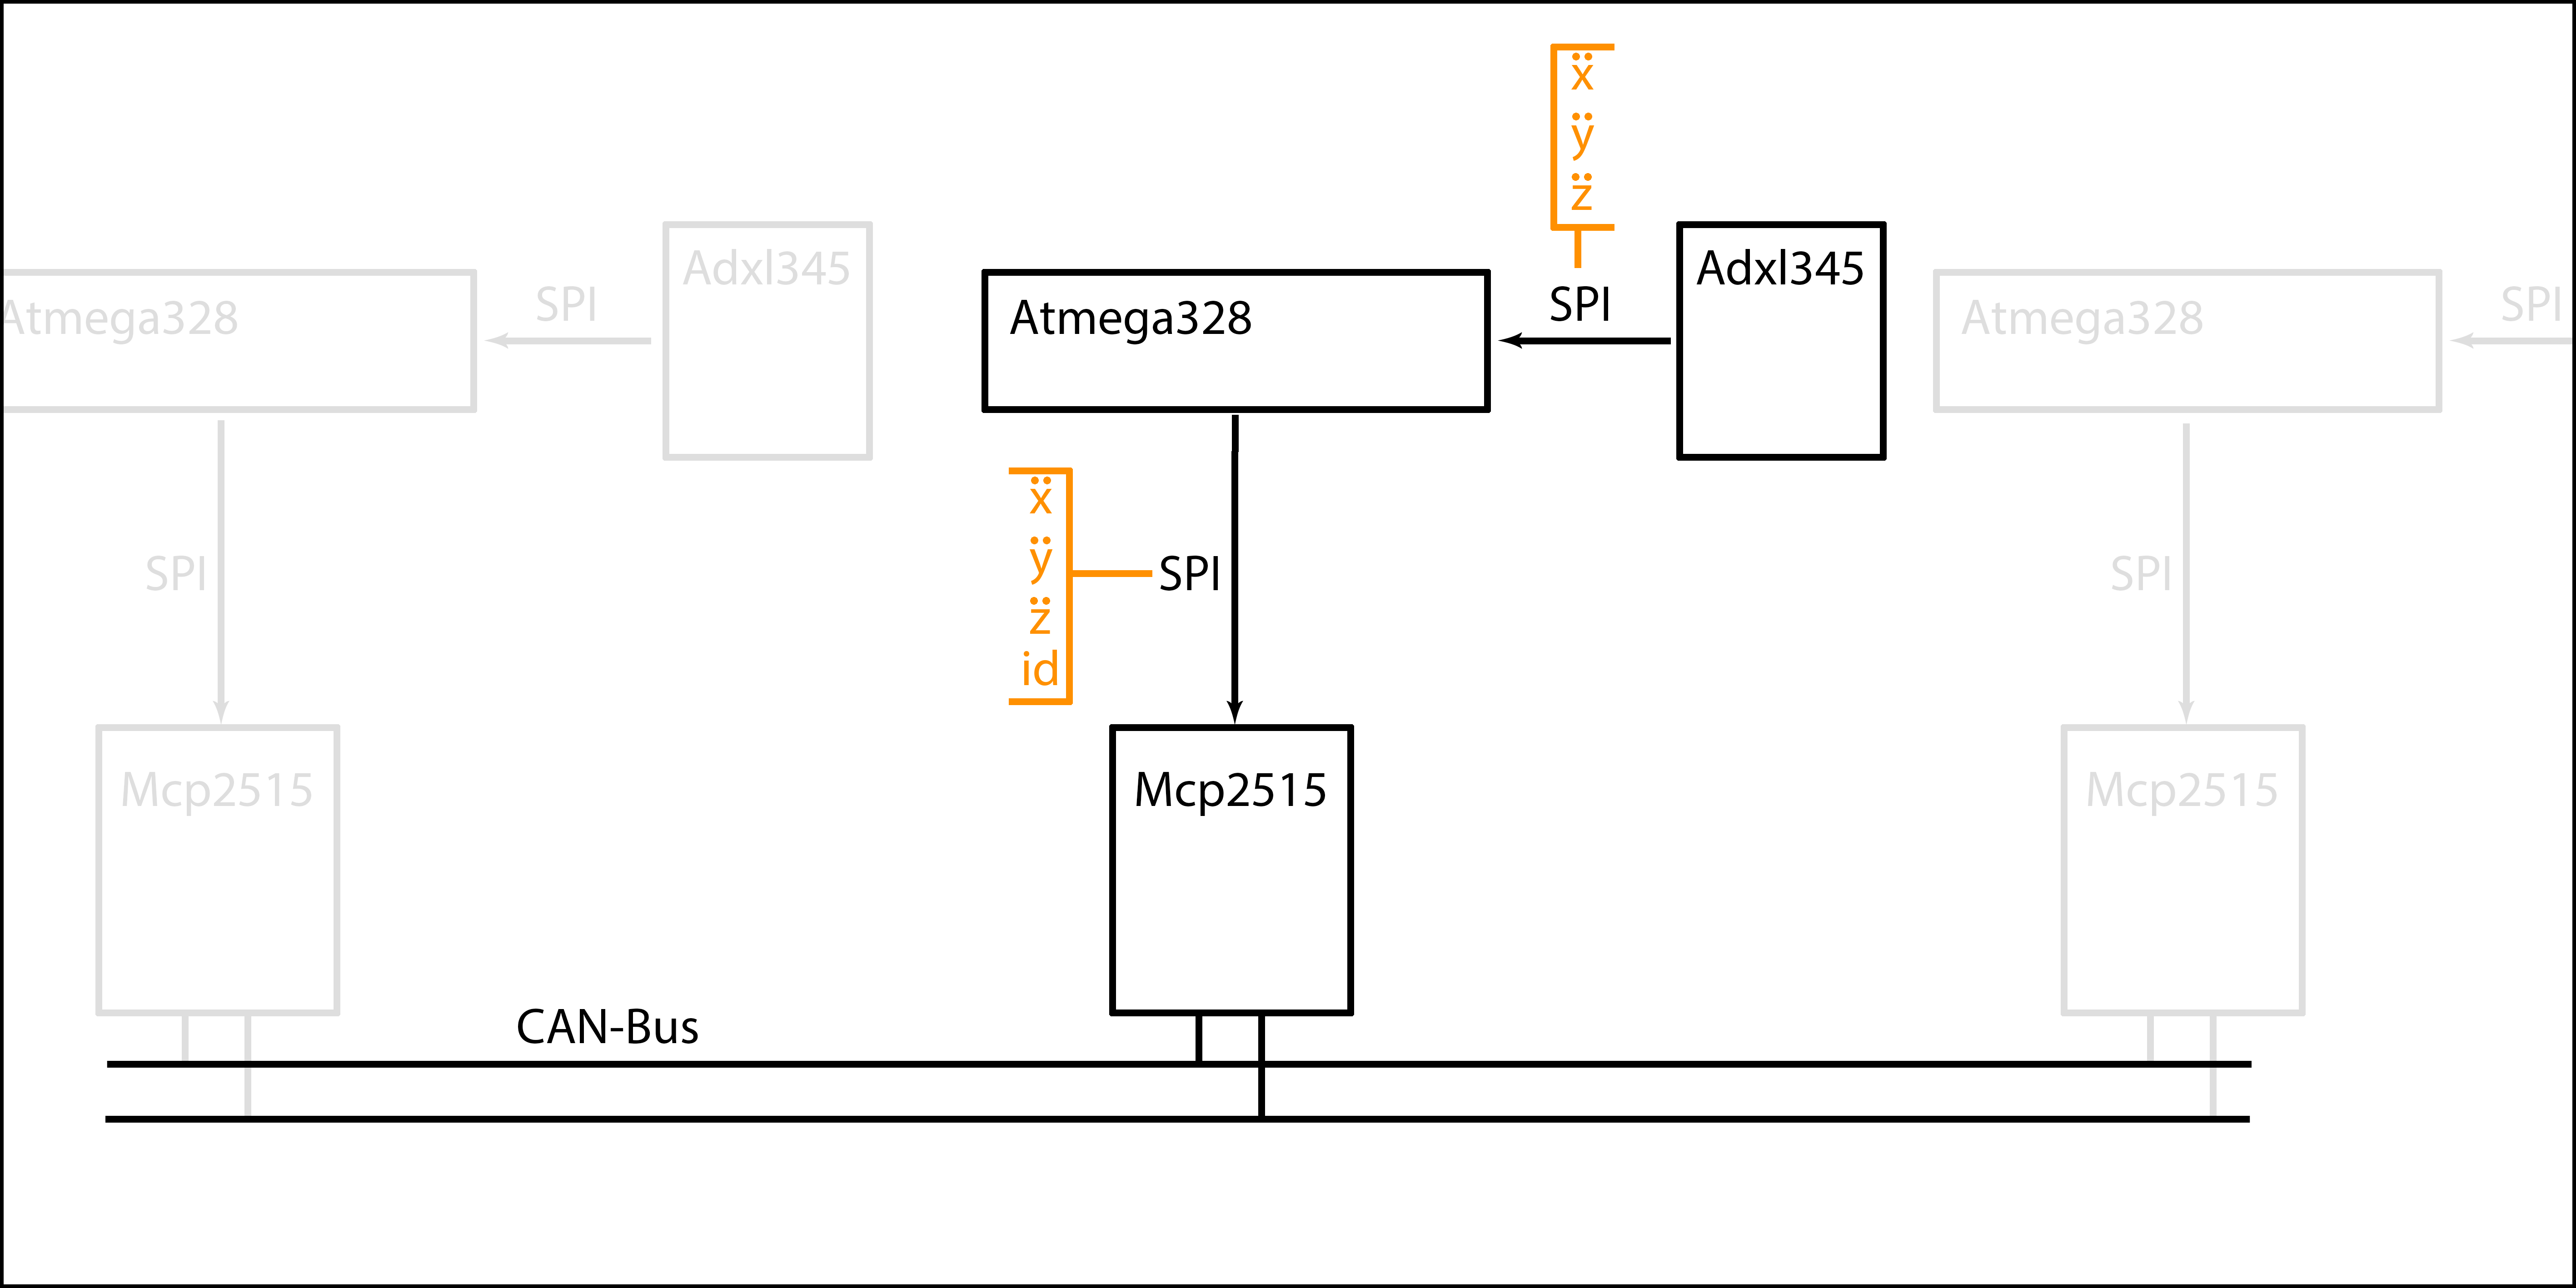
\includegraphics[width=1.0\linewidth]{03_Grafiken/Messsystem/Mcp2515EinheitZusammenspiel}
		\caption[Zusammenspiel der Komponenten Mcp-Executor-Einheit]{Zusammenspiel der Komponenten Mcp-Executor-Einheit}
		\label{fig:Mcp2515EinheitZusammenspiel}
	\end{figure}
	
Der Microcontroller Atmega328 lie�t von dem Beschleunigungssensor Adxl �ber die Schnittstelle SPI Sensordaten aus und gibt diese (ebenfalls �ber SPI) an den Mcp2515 weiter. Dieser schiebt die Daten auf den CAN-Bus.
	
\subsection{Verwendete Komponenten}
\label{kap:McpExecutorVerwendeteKomponenten}
F�r eine Einheit werden verschiedene Hardware-Komponenten verwendet, deren Wahl vor allem hinsichtlich des Kostenaufwandes erfolgte. Auch die Bauteilgr��e ist ein entscheidender Faktor, da die Einheiten m�glichst nicht st�rend sein sollen.

\begin{itemize}
	\item \textbf{Mcp2515}
	
	Der Mcp2515 beschreibt an sich den Chip, welcher auf der, in Abbildung \ref{fig:Mcp2515} dargestellten, Platine verbaut ist. Dieser Name wird jedoch f�r den gesamten Chip verwendet.
	\newline
	Die Funktion des Mcp2515 besteht darin Daten �ber die Schnittstelle SPI zu empfangen und �ber einen CAN-Bus zu versendet. Die Steuerung des Chips (z.B. Beschreiben eines Sende-Buffers) erfolgt dabei mit entsprechenden Kommandos �ber SPI. Das Konvertieren in L-, H-Pegel erfolgt komplett automatisch.
	
	\begin{figure}[H]
		\centering
		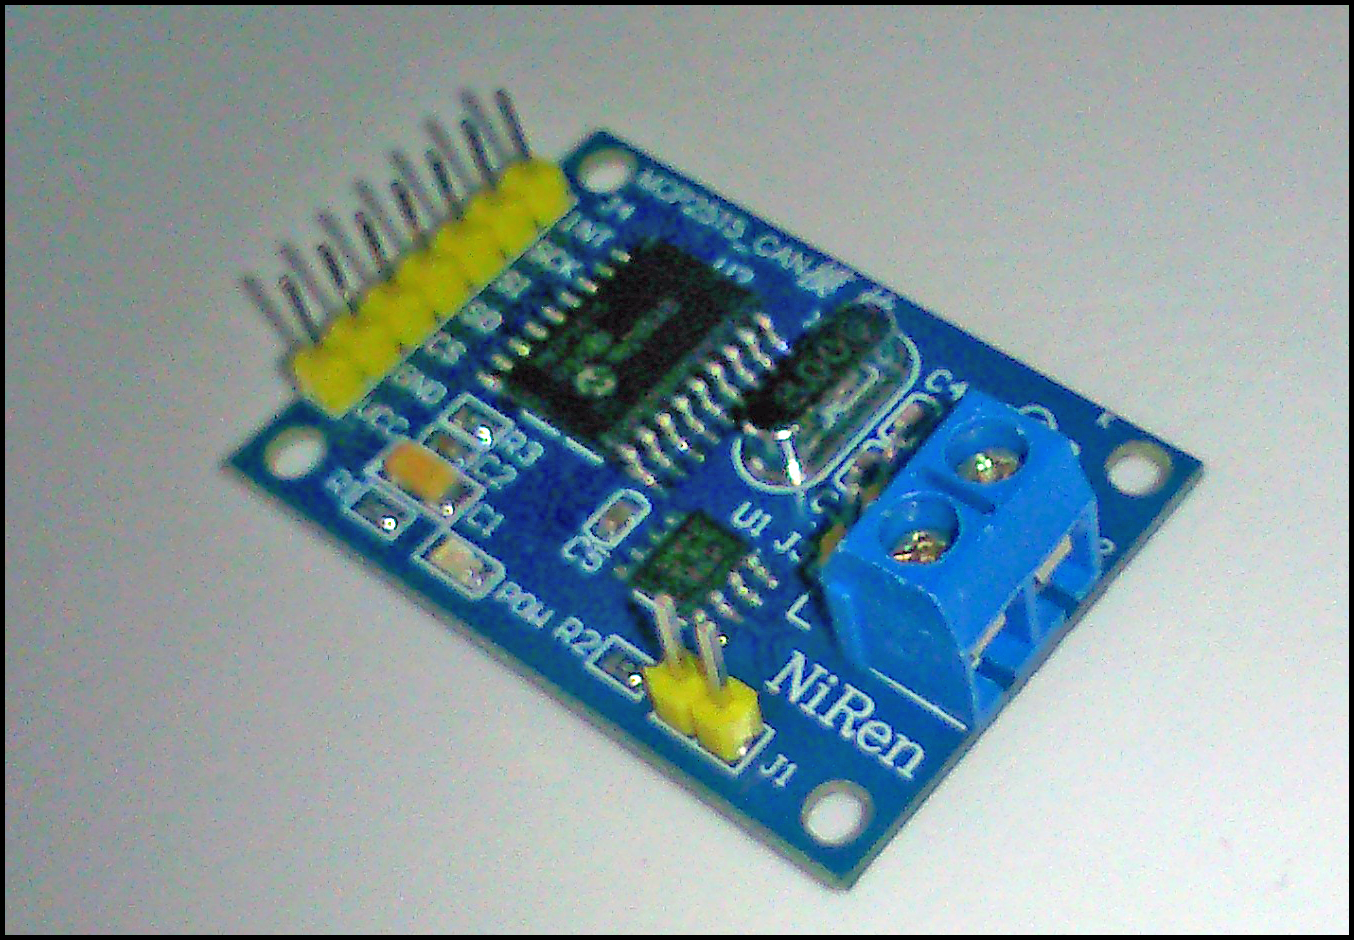
\includegraphics[width=0.4\linewidth]{03_Grafiken/Messsystem/Mcp2515}
		\caption[Mcp2515]{Mcp2515}
		\label{fig:Mcp2515}
	\end{figure}
	
	\item \textbf{Adxl345}
	
	Bei dem Adxl345 handelt es sich um einen 3-Achsen Beschleunigungssensor (s. Abbildung \ref{fig:Adxl345}), dessen Messwerte �ber SPI in verschiedenen Genauigkeiten ausgelesen werden k�nnen.
	Der Chip besitzt eine �u�erst geringe Leistungsaufnahme und ist kompatk in seiner Bauform.
		
	\begin{figure}[H]
		\centering
		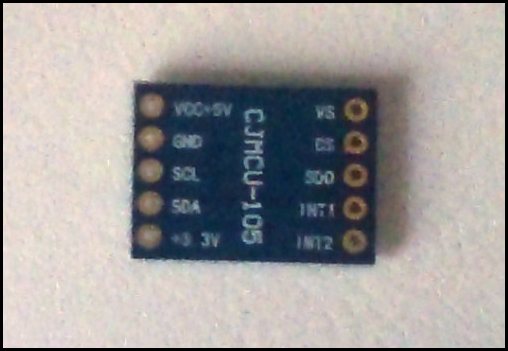
\includegraphics[width=0.4\linewidth]{03_Grafiken/Messsystem/Adxl345}
		\caption[Adxl345]{Adxl345}
		\label{fig:Adxl345}
	\end{figure}
	
	\item \textbf{Atmega328}
	
	Der Microcontroller Atmega328 ist u.A. in dem Arduino-Board verbaut. Es ist ein kostenf�nstiger Allrounder, welcher haupts�chlich wegen seiner gro�en Verbreitung gew�hlt wurde.
	Der Chip (s. Abbildung \ref{fig:Atmega328}) besitzt eine SPI-Schnittstelle und diverse I/O's, weshalb die Projektanforderungen vollst�ndig erf�llt werden.
	\newline
	Es exisiteren zwei verschiedene Versionen des MCU's, von denen die Atmega328-P Variante f�r eine geringe Leistungsaufnahme konzipiert ist. 
	
	\begin{figure}[H]
		\centering
		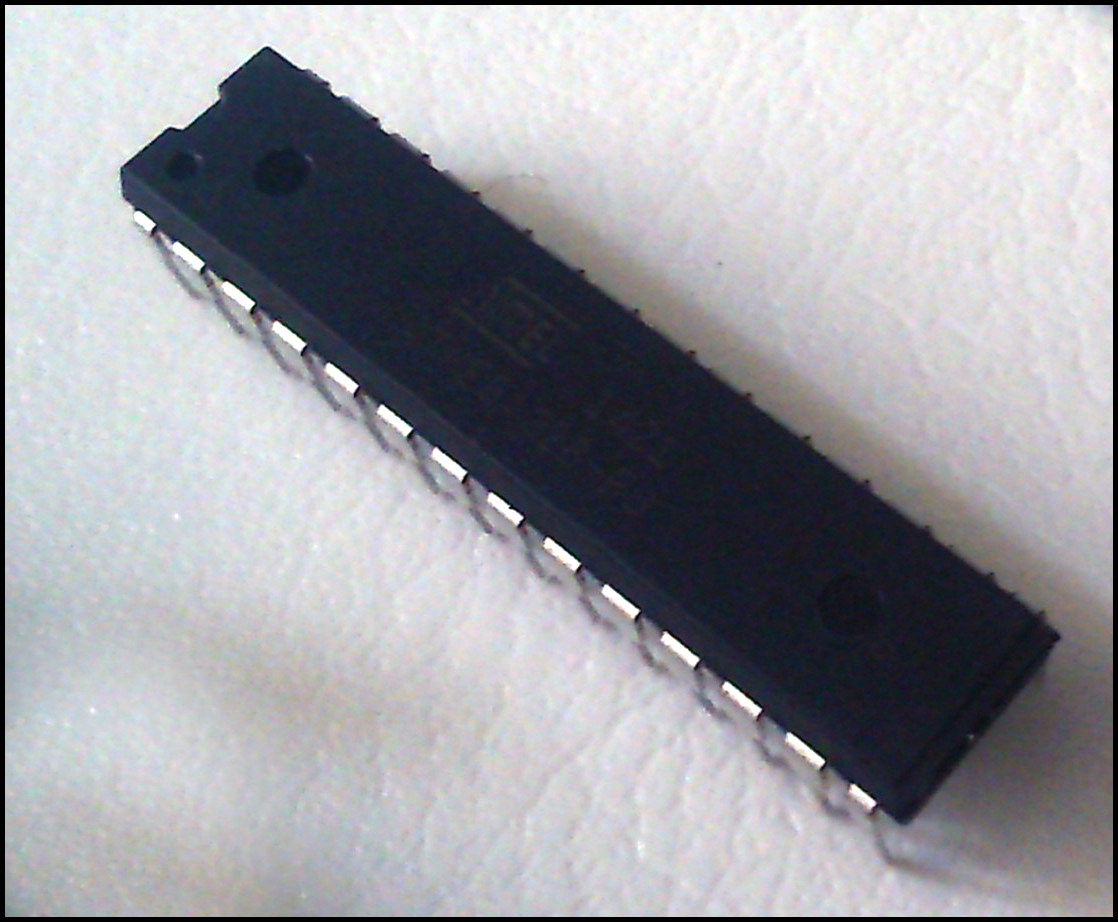
\includegraphics[width=0.4\linewidth]{03_Grafiken/Messsystem/Atmega328}
		\caption[Atmega328]{Atmega328}
		\label{fig:Atmega328}
	\end{figure}
	
	\item \textbf{Oscillator und Kondensator}
	
	Der Atmega328 ben�tigt einen externen Taktgeber, welcher mit einem 16Mhz Quarz und entsprechenden Kondensatoren gew�hlt wird (s. Abbildung \ref{fig:Oscillator}).
	
	\begin{figure}[H]
		\centering
		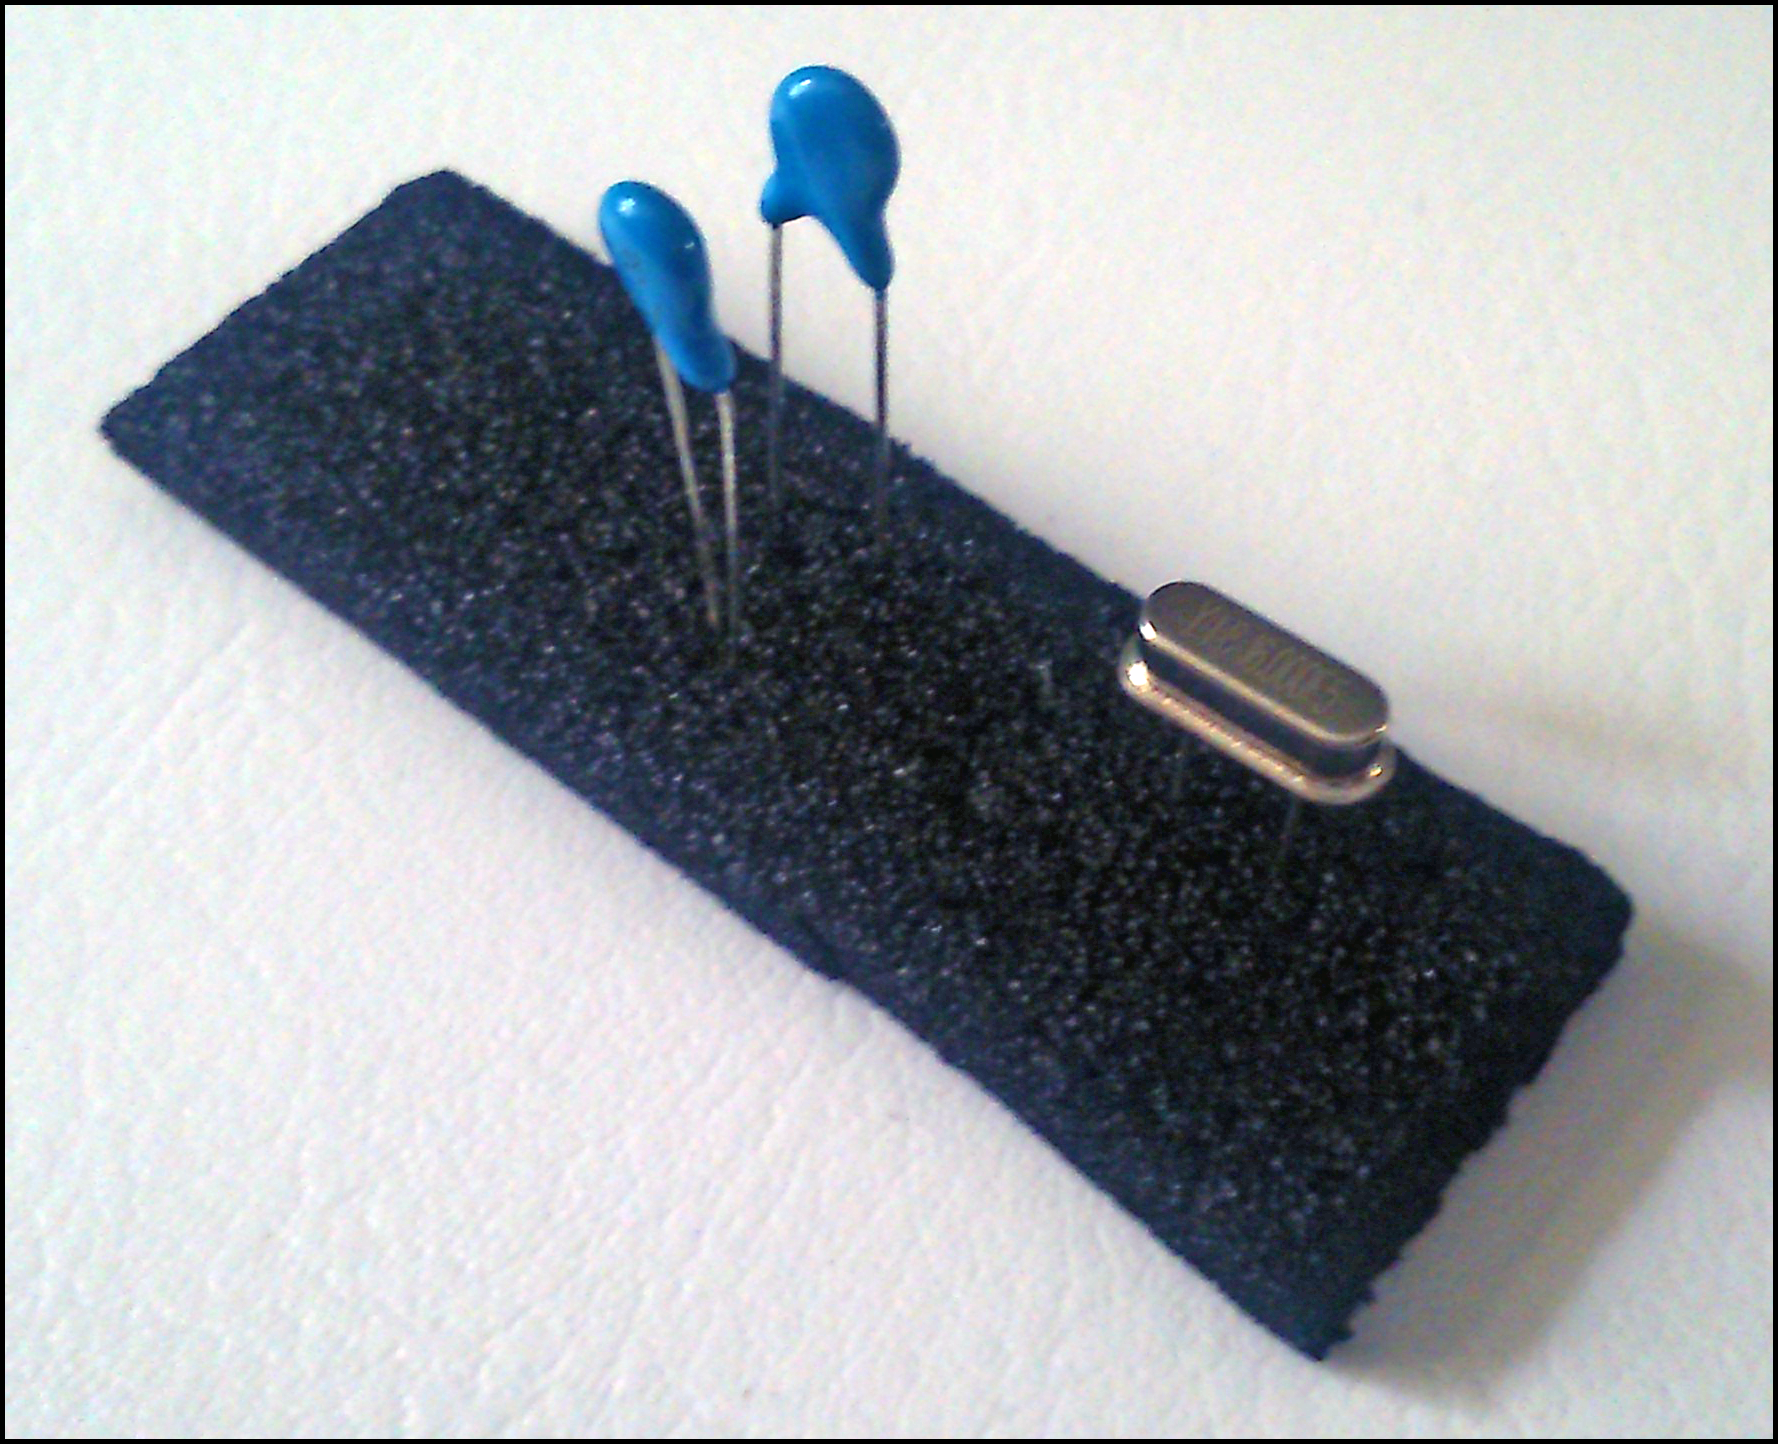
\includegraphics[width=0.4\linewidth]{03_Grafiken/Messsystem/Oscillator}
		\caption[Oscillator]{Oscillator}
		\label{fig:Oscillator}
	\end{figure}
		
\end{itemize}
\subsection{Testversion}
\label{kap:McpExecutorTestversion}
Um die Funktionen der Chips zu verstehen und beherrschen zu k�nnen erfolgt der Aufbau einer Einheit auf einem Entwicklungsboard (Whiteboard). Dieser Aufbau beinhaltet alles, was f�r eine Einheit vorgesehen ist, d.h. einen Atmega328 (mit externem Taktgeber), einen Adxl345 und einen Mcp2515. Mit entsprechender Verdrahtung (s. Schaltbild \ref{fig:SchaltbildEinheit}) und der Entwicklung eines Programms, welches auf der MCU aktiv ist, lassen sich die Sensorwerte �ber einen CAN-Bus auslesen. Die Sensor-ID muss programmatisch auf der MCU definiert werden. 

\begin{figure}[H]
	\centering
	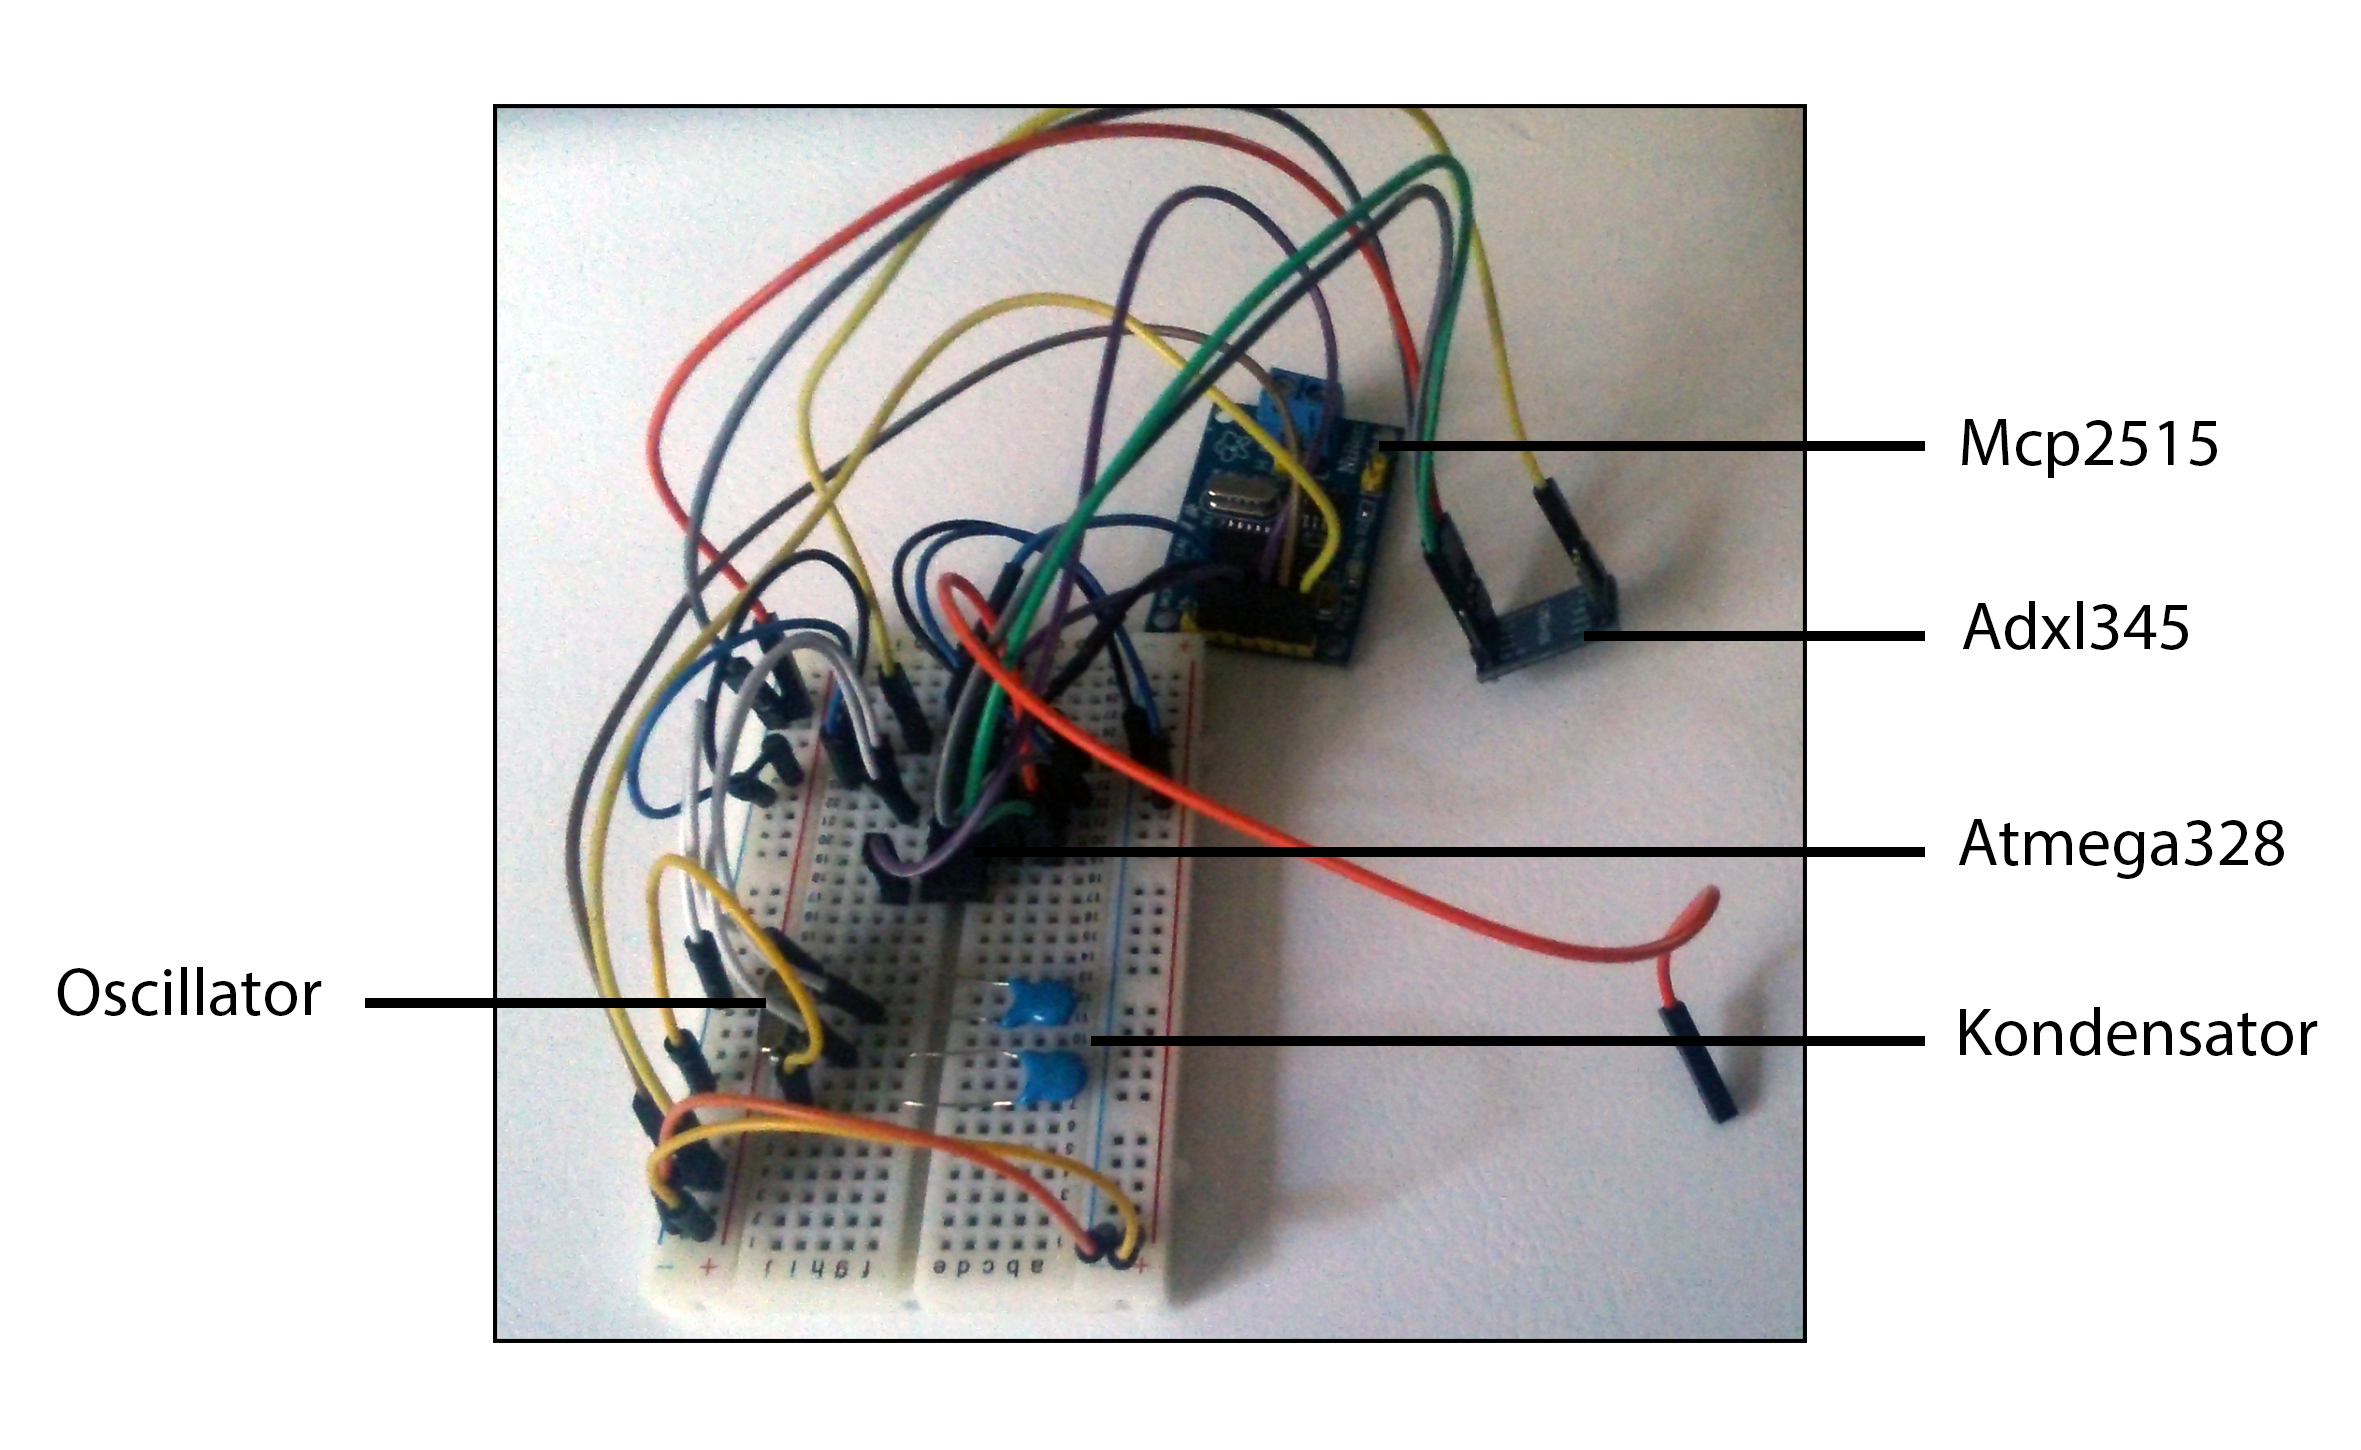
\includegraphics[width=0.9\linewidth]{03_Grafiken/Messsystem/McpExecutorTest}
	\caption[Testversion einer Mcp-Executor-Einheit]{Testversion einer Mcp-Executor-Einheit}
	\label{fig:McpExecutorTest}
\end{figure}

Mit zwei solcher Testaufbauten wurde das Aufnehmen von Sensorwerten validiert.
\subsection{Beta version}
\label{kap:McpExecutorBetaversion}
F�r die Betaversion der Mcp-Executor-Einheit werden alle Komponenten in ein Geh�use integriert (s. Abbildung \ref{fig:McpExecutorBeta}), welches gerade so gro� ist, dass es beim Tragen am K�rper m�glichst nicht st�rt und einfach befestigt werden kann. F�r das Integrieren werden zus�tliche Platinen angefertigt.
\newline
Aufgrund des Feststellens verschiedener negativer Aspekte w�hrend der Entstehung der Einheiten existieren mehrere Beta-Versionen, von denen jedoch nur die erste aufgeziegt wird.

\begin{figure}[H]
	\centering
	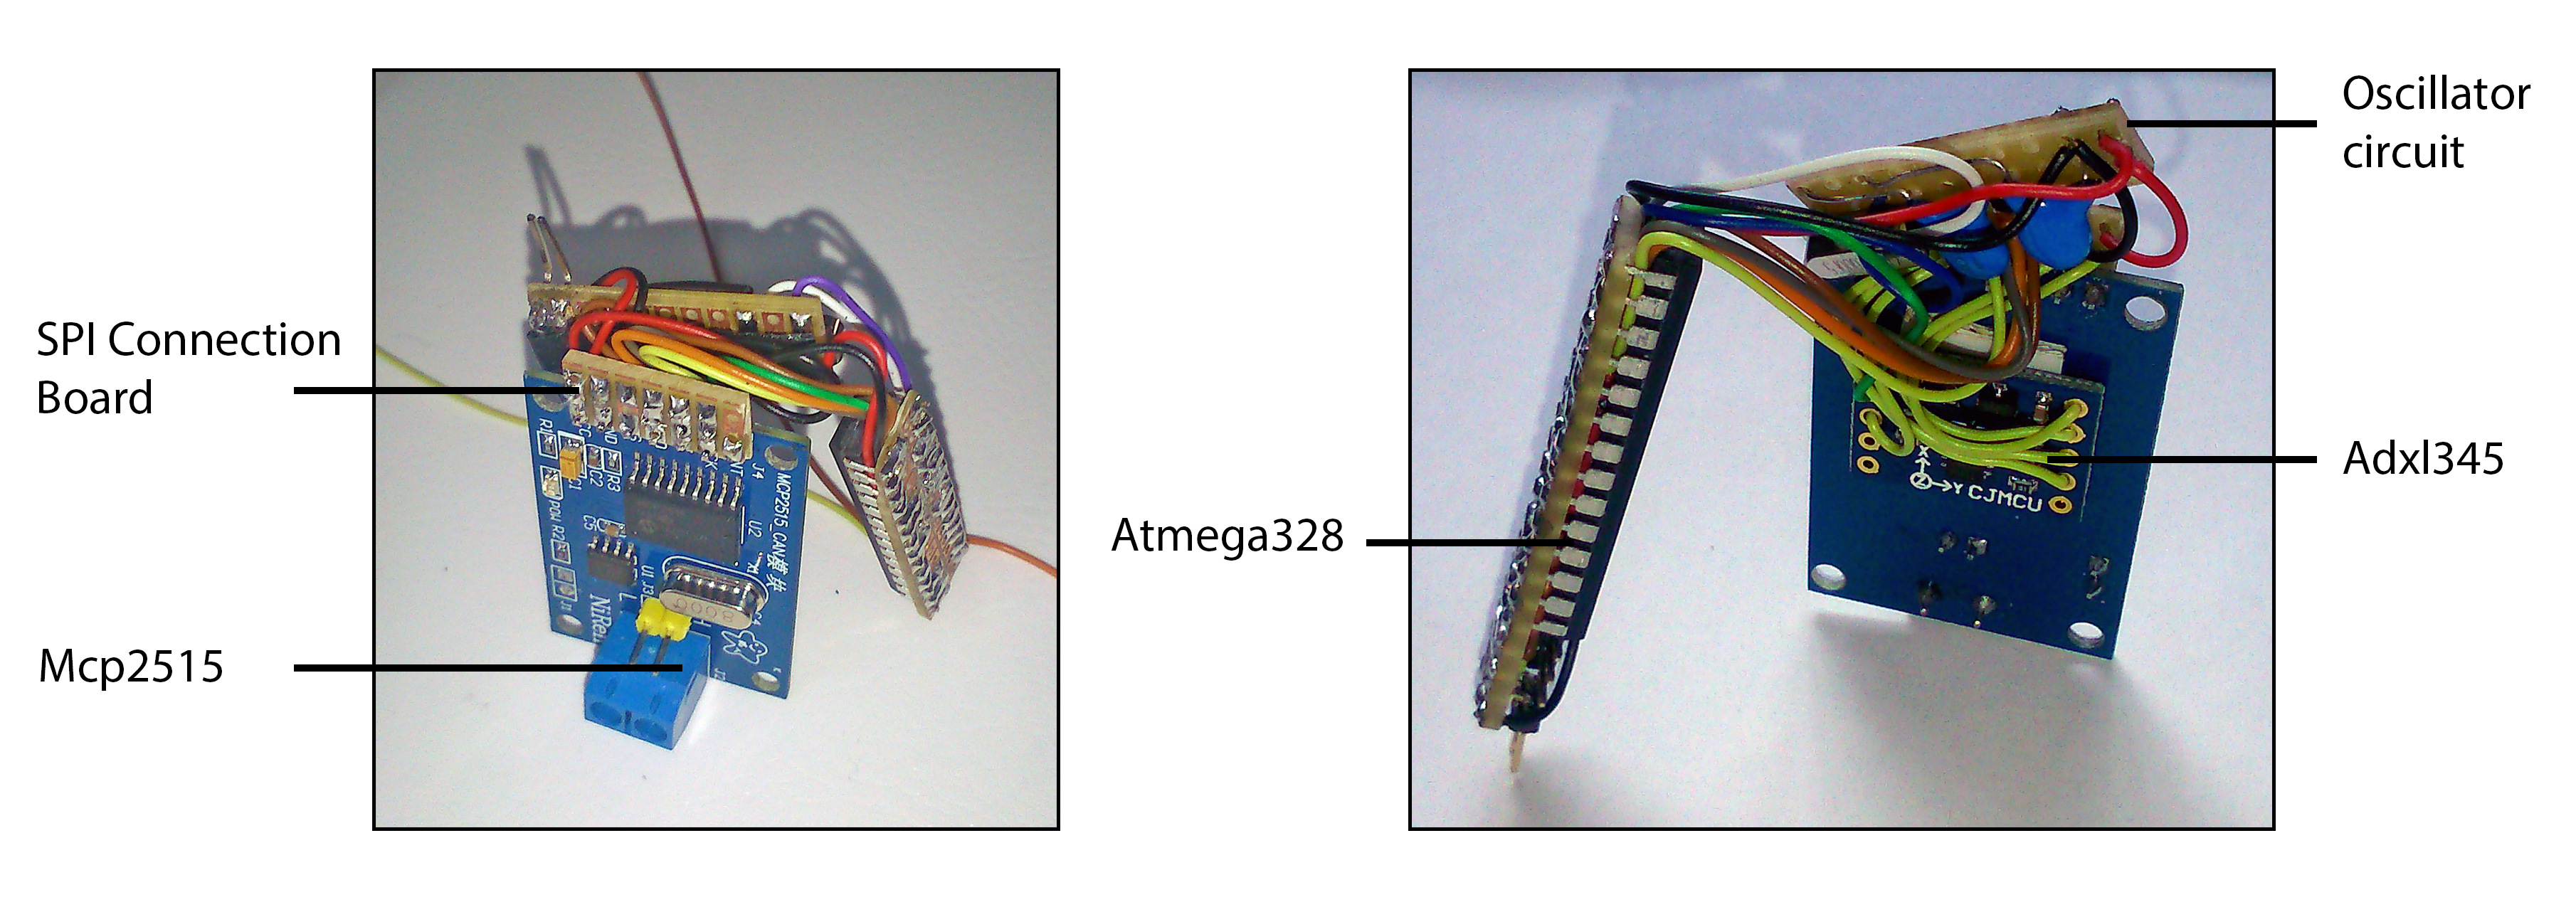
\includegraphics[width=1.0\linewidth]{03_Grafiken/Messsystem/McpExecutor_BetaDetail}
	\caption[Betaversion einer Mcp-Executor-Einheit]{Betaversion einer Mcp-Executor-Einheit}
	\label{fig:McpExecutorBeta}
\end{figure}

Die Befestigung der Einheit am K�rper erfolgt anhand eines Positioniergurtes. Dieser besteht in der ersten Beta-Version aus zwei und Klettverschl�ssen, die an dem Abdeckblech der Einheit befestigt sind. Durch ein entsprechendes Gegenst�ck des Klettverschlusses auf der R�ckseite des Abdeckblechs ist der notwendige Halt gegeben.\\
An dem Anzug sind ebenfalls entsprechende Gegenst�cke des Klettverschlusses angebracht, sodass die Einheiten w�hrend der Bewegung nicht verrutschen. 

%
% BILD KLETTVERSCHLUSS
%
\begin{figure}[H]
	\centering
	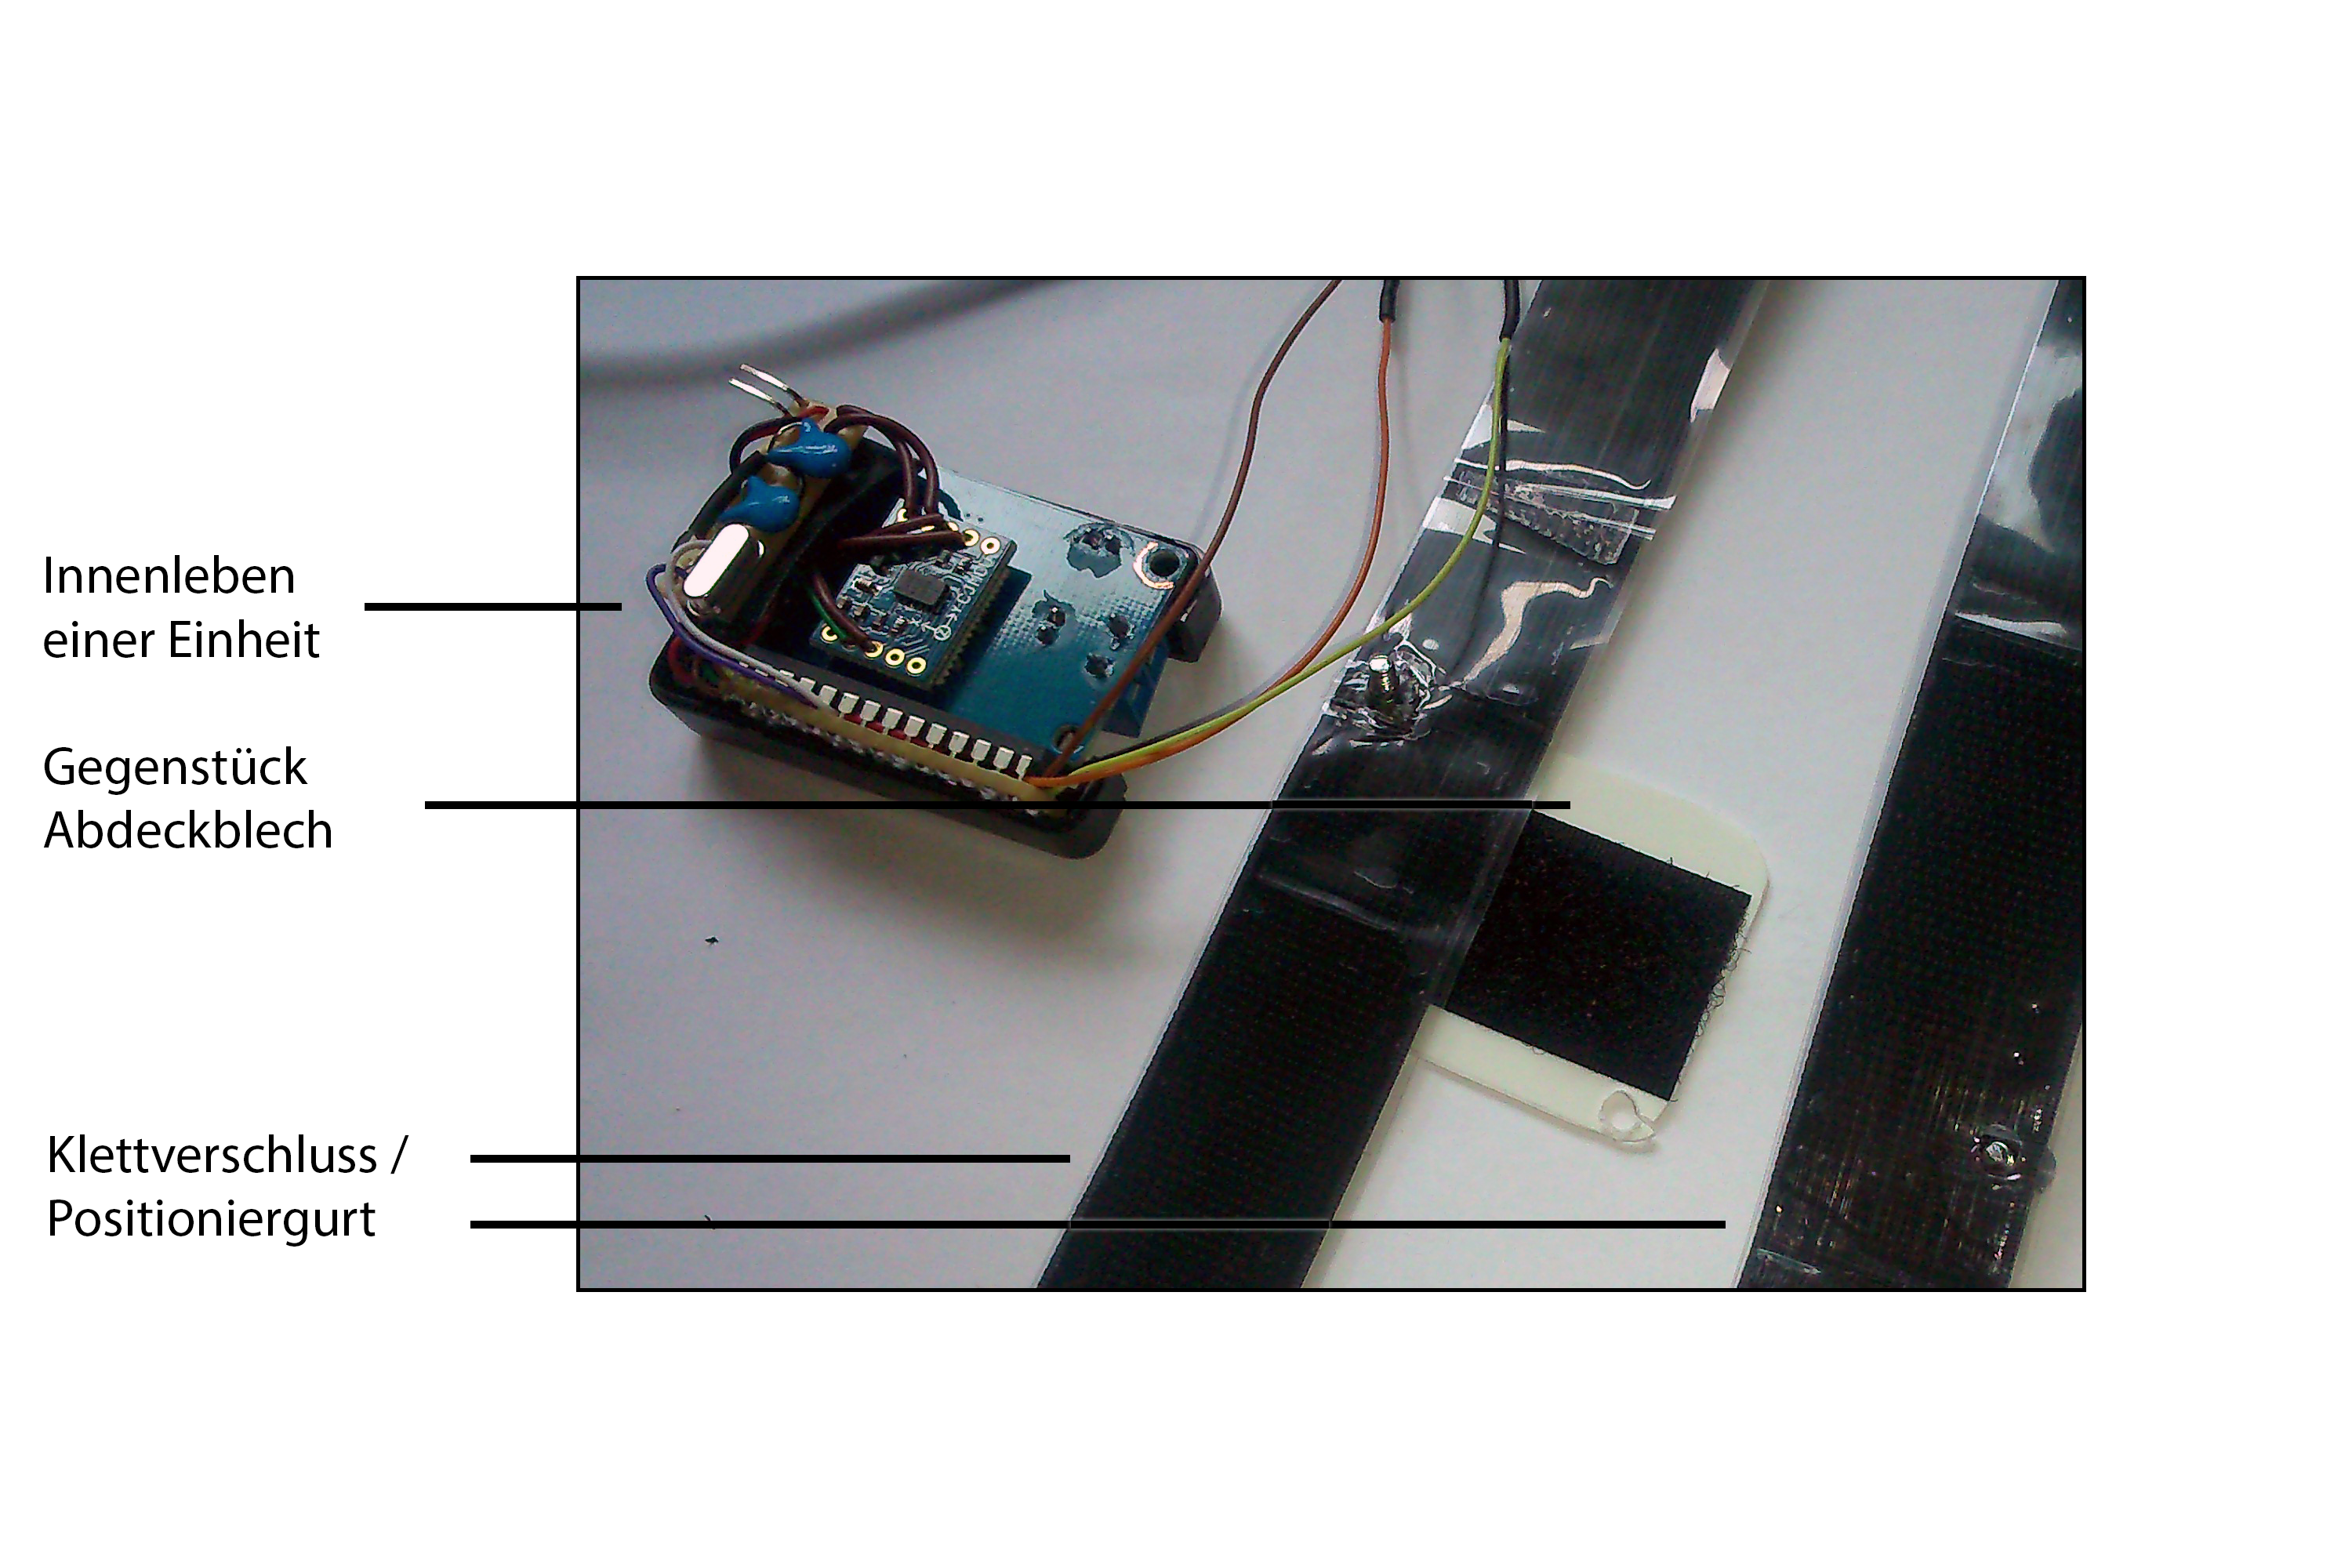
\includegraphics[width=1.0\linewidth]{03_Grafiken/Messsystem/McpExecutor2515Klettverschluss}
	\caption[Betaversion einer Mcp-Executor-Einheit - Klettverschluss]{Betaversion einer Mcp-Executor-Einheit - Klettverschluss}
	\label{fig:McpExecutorBetaKlettverschluss}
\end{figure}




\subsection{Release version}
\label{kap:McpExecutorReleaseversion}
Bei der Realease-Version der Mcp-Executor-Einheit wird die Beta-Version zun�chst bewertet und alle negativen Aspekte aufgezeigt und m�gliche L�sungen erarbeitet. Die zu verbessernden Punkte sind in Tabelle \ref{tab:McpExecutorEinheitNegAspekte} aufgelistet:

 
%\begin{figure}[H]
%	\centering
%	\includegraphics[width=0.7\linewidth]{03_Grafiken/Messsystem/McpExecutorRelease}
%	\caption[Release-Version einer Mcp-Executor-Einheit]{Release-Version einer Mcp-Executor-Einheit}
%	\label{fig:McpExecutorRelease}
%\end{figure}
%\subsection{Programmaufbau}
\label{kap:McpExecutorProgrammaufbau}
\begin{enumerate}
	%
	% Setup-Routine
	%
	\item \textbf{Setup-Routine}\\
	% LISTING F�R SETUP() 
	Das Programm, welches auf der \gls{MCU} einer Einheit aktiv ist besteht aus einer Setup- und einer Loop-Routine. Innerhalb des Setups efolgt die Definition verschiedener Variablen und die Konfiguration der SPI-Schnisttstelle, sowie der Komponenten Adxl345 und Mcp2515 (s. Listing \ref{lst:mcpExecutorSetup}).
	In den Zeilen 4-6 und 8-10 werden die Ausg�nge zum Ausw�hlen der Ger�te, entsprechend der SPI-Schnittstelle, gesetzt. Dabei ist zu beachten, dass bei der Atmega-\gls{MCU} der Ausgang an Pin 10 immer immer gesetzt werden muss, auch wenn ein anderer Pin als Device-Selector verwendet wird. Der SIgnalzustand der Pins muss HIGH entsprechen, da bei einem Low-Pegel das entsprechende Ger�t ausgew�hlt wird.\\
	Zeile 12-13 initialisiert die SPI-Schnittstelle mit 5 Mhz und dem SPI-Mode 3 (CPOL = 1, CPHA = 1). Diese einzig verf�gbare Einstellung richtet sich nach dem Beschleunigungssensor Adxl345. Mit dem Aufruf der Routine SPI.begin() beginnt die Verwendung der Schnittstelle, sodass in den Zeilen 15-16 die Initialisierungsdaten an die Ger�te gesendet werden k�nnen. Diese beinhalten f�r den Sensor Adxl345 u.A. das Datenformat und f�r den Mcp2515 das CAN-Bus Setup. F�r das CAN-Bus Setup ist zu beachten, dass die Nachrichten jedes Teilnehmers einen spzifischen Identifier aufweisen muss.\\
	\input{02_Inhalt/Messsystem/Listings/mcpExecutorSetup}
	%
	% Loop-Routine
	%
	\item \textbf{Loop-Routine}\\
	In der Loop-Routine (s. Listing \ref{lst:mcpExecutorLoop}) werden zwei Methoden aufgerufen, von denen die Prozedur \textit{getAdxlData()} die Sensordaten lie�t und zusammen mit einem Zeitstempel in ein Array speichert.
	Die Routine \textit{mcp2515\_load\_tx\_buffer()} schreibt die Daten nacheinander in die Sende-Buffer 1-3.\\
	Innerhalb der Routine \textit{getAdxlData()} erfolgt in Zeile 10 das Setzen der entsprechenden Registerwerte, um die Sensordaten auslesen zu k�nnen. In den Zeilen 12-15 erfolgt das Auslesen, indem der Selektor-Pin auf Low-Level gelegt wird. Anschlie�end erfolgt das Senden von 0-Werten, um per SPI die Sensordaten auszulesen (f�r jede Achse zwei Byte). In Zeile 17 wird noch die ID f�r das Ger�t angegeben.\\
	Innerhalb der Routine mcp2515\_load\_tx\_buffer0() erfolgt in den Zeilen 25-47 das Setzen der Registeradresse eines Sendebuffers, in Abh�ngigkeit welcher zuletzt genutzt wurde. In Zeile 51 werden in den ausgew�hlten Sendebuffer die Sensordaten gelegt und mit dem in Zeile 53 angegebenen Kommando auf den CAN-Bus geschickt.
	\input{02_Inhalt/Messsystem/Listings/mcpExecutorLoop}

\end{enumerate}

\section{Hauptrechner}
\label{kap:Hauptrechner}
Der Hauptrechner definiert ein Ger�t, welches als Master die Sensordaten aller Mcp-Executor-Einheiten anfordert und verarbeitet.  

\subsection{Verwendete Komponenten}
\label{kap:HauptrechnerVerwendeteKomponenten}
Die Bestandteile des Hauptrechners sind ein Raspberry-Pi 2 mit Wlan-Adapter und dem Betriebsystem Windows 10 IoT, sowie einer Energiequelle (Akku von Anker) mit 20100 mAh. F�r das Konvertieren der Sensordaten von CAN auf SPI wird, in ein Geh�use integriertes, Mcp2515 verwendet.

\begin{itemize}
	\item \textbf{Raspberry-Pi 2}
	
	Der Raspberry Pi 2 (s. Abbildung \ref{fig:Raspberry}) ist in seiner zweiten Version ein stabiles System, welches in Verbindung mit Windows IoT in der HOchsprache C\# programmiert werden kann. Die Programme entsprechen den Anwendungen wie man sie von Smartphones kennt.
	\newline
	Die zweite Version beinhaltet (im Vergleich zur Version 3) keinen Wlan-Adapter, weshalb dieser zus�tzlich erworben werden muss.
	
	\begin{figure}[H]
		\centering
		
\includegraphics[width=0.7\linewidth]{03_Grafiken/pseudoImage}
		\caption[Raspberry Pi 2]{Raspberry Pi 2}
		\label{fig:Raspberry}
	\end{figure}

	\item \textbf{Wlan-Adapter}
	
	Bei der Wahl eines Wlan-Adapters muss die Kompatibilit�t zu Windows-IoT ber�cksichtigt werden, da nicht f�r jedes Ger�t entsprechende Treiber zur Verf�gung stehen. Aus diesem Grunde liegt die Wahl bei dem preisg�nstigen Wlan-Adapter XXXX (s. Abbildung \ref{fig:Adxl345}).
	
	\begin{figure}[H]
		\centering
		
\includegraphics[width=0.7\linewidth]{03_Grafiken/pseudoImage}
		\caption[Wlan Adapter]{Wlan Adapter}
		\label{fig:WlanAdapter}
	\end{figure}
	
	\item \textbf{Akku von Anker}
	
	F�r die Energieversorgung (s. Abbildung \ref{fig:Anker}) wird ein Akku ben�tigt, welcher eine hohe Kapazit�t aufweist und gen�gend Strom liefert, damit das System ordnungsgem�� funktioniert. Bspw. ben�tigt der Raspberry Pi 2 2A, um einen fehlerfreien Betrieb zu gew�hrleisten (mit zus�tzlich angeschlossener Hardware, wie z.B. der Wlan-Adapter).  
	\newline
	Der Akku PowerCore 20100 von Anker ist f�r diese Anforderungen wie geschaffen, da dieser 20100 mAh aufweist und 2 USB-Ports mit jeweils 2A zur Verf�gung stellt.
		
	\begin{figure}[H]
		\centering
		
\includegraphics[width=0.7\linewidth]{03_Grafiken/pseudoImage}
		\caption[Akku Anker]{Akku Anker}
		\label{fig:Anker}
	\end{figure}
	
		\item \textbf{Mcp2515 mit Geh�use}
		
		Pseudotext Pseudotext Pseudotext Pseudotext Pseudotext Pseudotext Pseudotext Pseudotext Pseudotext Pseudotext Pseudotext Pseudotext Pseudotext Pseudotext Pseudotext 
	
\end{itemize}
\subsection{Release Version}
\label{kap:HauptrechnerReleaseVersion}
Pseudotext Pseudotext Pseudotext Pseudotext Pseudotext Pseudotext Pseudotext Pseudotext Pseudotext Pseudotext Pseudotext Pseudotext Pseudotext Pseudotext Pseudotext Pseudotext Pseudotext Pseudotext Pseudotext Pseudotext Pseudotext Pseudotext Pseudotext Pseudotext Pseudotext Pseudotext Pseudotext Pseudotext Pseudotext Pseudotext Pseudotext Pseudotext Pseudotext Pseudotext Pseudotext Pseudotext Pseudotext Pseudotext Pseudotext Pseudotext 
\subsection{Programmaufbau}
\label{kap:HauptrechnerProgrammaufbau}
Pseudotext Pseudotext Pseudotext Pseudotext Pseudotext Pseudotext Pseudotext Pseudotext Pseudotext Pseudotext Pseudotext Pseudotext Pseudotext Pseudotext Pseudotext Pseudotext Pseudotext Pseudotext Pseudotext Pseudotext Pseudotext Pseudotext Pseudotext Pseudotext Pseudotext Pseudotext Pseudotext Pseudotext Pseudotext Pseudotext Pseudotext Pseudotext Pseudotext Pseudotext Pseudotext Pseudotext Pseudotext Pseudotext Pseudotext Pseudotext 

\section{Anzug}
\label{kap:Anzug}
Pseudotext Pseudotext Pseudotext Pseudotext Pseudotext Pseudotext Pseudotext Pseudotext Pseudotext Pseudotext Pseudotext Pseudotext Pseudotext Pseudotext Pseudotext Pseudotext Pseudotext Pseudotext Pseudotext Pseudotext Pseudotext Pseudotext Pseudotext Pseudotext Pseudotext Pseudotext Pseudotext Pseudotext Pseudotext Pseudotext Pseudotext Pseudotext Pseudotext Pseudotext Pseudotext Pseudotext Pseudotext Pseudotext Pseudotext Pseudotext 

\subsection{Verwendete Komponenten}
\label{kap:AnzugVerwendeteKomponenten}
Pseudotext Pseudotext Pseudotext Pseudotext Pseudotext Pseudotext Pseudotext Pseudotext Pseudotext Pseudotext Pseudotext Pseudotext Pseudotext Pseudotext Pseudotext Pseudotext Pseudotext Pseudotext Pseudotext Pseudotext Pseudotext Pseudotext Pseudotext Pseudotext Pseudotext Pseudotext Pseudotext Pseudotext Pseudotext Pseudotext Pseudotext Pseudotext Pseudotext Pseudotext Pseudotext Pseudotext Pseudotext Pseudotext Pseudotext Pseudotext 
\subsection{Testversion}
\label{kap:AnzugTestversion}
Pseudotext Pseudotext Pseudotext Pseudotext Pseudotext Pseudotext Pseudotext Pseudotext Pseudotext Pseudotext Pseudotext Pseudotext Pseudotext Pseudotext Pseudotext Pseudotext Pseudotext Pseudotext Pseudotext Pseudotext Pseudotext Pseudotext Pseudotext Pseudotext Pseudotext Pseudotext Pseudotext Pseudotext Pseudotext Pseudotext Pseudotext Pseudotext Pseudotext Pseudotext Pseudotext Pseudotext Pseudotext Pseudotext Pseudotext Pseudotext 
\subsection{Beta version}
\label{kap:AnzugBetaversion}
Pseudotext Pseudotext Pseudotext Pseudotext Pseudotext Pseudotext Pseudotext Pseudotext Pseudotext Pseudotext Pseudotext Pseudotext Pseudotext Pseudotext Pseudotext Pseudotext Pseudotext Pseudotext Pseudotext Pseudotext Pseudotext Pseudotext Pseudotext Pseudotext Pseudotext Pseudotext Pseudotext Pseudotext Pseudotext Pseudotext Pseudotext Pseudotext Pseudotext Pseudotext Pseudotext Pseudotext Pseudotext Pseudotext Pseudotext Pseudotext 
\subsection{Release version}
\label{kap:AnzugReleaseversion}
Pseudotext Pseudotext Pseudotext Pseudotext Pseudotext Pseudotext Pseudotext Pseudotext Pseudotext Pseudotext Pseudotext Pseudotext Pseudotext Pseudotext Pseudotext Pseudotext Pseudotext Pseudotext Pseudotext Pseudotext Pseudotext Pseudotext Pseudotext Pseudotext Pseudotext Pseudotext Pseudotext Pseudotext Pseudotext Pseudotext Pseudotext Pseudotext Pseudotext Pseudotext Pseudotext Pseudotext Pseudotext Pseudotext Pseudotext Pseudotext 

\section{Erfassungsprogramm}
\label{kap:Erfassungsprogramm}
Das Lesen, bzw. Speichern der Sensordaten erfolgt mit einem Programm, welches sich als Client mit dem Server verbindet und �ber WLAN die Daten aller Sensoren empf�ngt. Die Sensorwerte werden nicht automatisch gespeichert, jedoch empfangen und k�nnen grafisch dargestellt werden (x-, y-, z-Werte f�r jeden Sensor in einer �bersicht). Ist das Speichern der Daten gew�nscht, so muss eine Anzahl an Samples angegeben werden. Das Speichern der Daten erfolgt dann in eine Datenbank.

\subsection{Beschreibung HMI - Main}
\label{kap:ClientGraphProgramm}
Die HMI gliedert sich in mehrere Bereiche, in denen verschiedene Funktionalit�ten bereitgestellt werden. Diese finden im folgenden Abschnitt Erl�uterung. 

\begin{figure}[H]
\centering
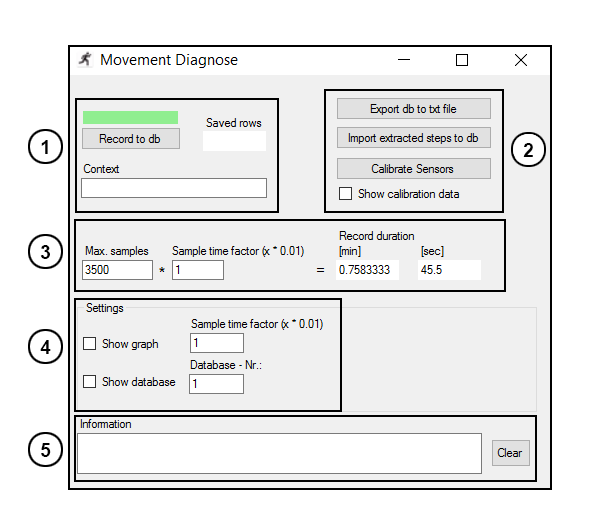
\includegraphics[width=1.0\linewidth]{03_Grafiken/Messsystem/ClientGraph_Gui}
\caption[Client Graph HMI]{Client Graph HMI}
\label{fig:clientgraphgui}
\end{figure}

\begin{enumerate}
	\item \textbf{Aufnahme starten} \\
	Der gr�ne Balken dient als Indikator, ob Messwerte empfangen werden (gr�n: Messung kann gestartet werden, rot: Es werden keine Daten empfangen).\\
	Durch das Bet�tigen des Buttons \textit{Record to db} wird eine Messung gestartet bis diese abgebrochen oder die max. Anzahl an Samples erreicht wird.\\
	Das Label \textit{Saved rows} zeigt die aktuelle Anzahl aufgenommener Messwerte an.\\
	Im Textfeld \textit{Context} kann eine Bezeichnung der Messwerte eingegeben werden (die exportierten Textdateien tragen diesen Namen).
	
	\item \textbf{Import / Export und Kalibrierung}\\
	Mit dem Bet�tigen des Buttons \textit{Export...} erfolgt das Exportieren der erfassten Sensordaten in eine CSV-Datei. Jeder Sensor generiert eine eigene Datei mit dem unter \textit{Context} angegebenen Namen.\\
	Durch das Bet�tigen des Buttons \textit{Import...} kann eine Textdatei (CSV-Format) eingelesen und in die Datenbank geschrieben werden.\\
	Durch das Bet�tigen des Buttons \textit{Calibrate Sensors} erfolgt das Kalibrieren aller Sensoren (s. Beschreibung in \ref{kap:Erfassungsprogramm}). Durch das Setzen des H�kchens \textit{Show...} erfolgt das Darstellen der kalibrierten Sensorwerte.
	
	\item \textbf{Aufnahmezeit}\\
	In das Textfeld \textit{Max. samples} wird die aufzunehmende Anzahl an Messwerten eingetragen. Danach stoppt die Messung automatisch. Standardm��ig sind 3500 Samples eingetragen, da bei einer zu gro�en Anzahl eine \textit{Out of memory Exception} geworfen wird.
	
	\item \textbf{Settings}\\
	Durch das Setzen des H�kchens bei \textit{Show graph} werden die Sensorwerte visualisiert.\\
	Durch das Setzen des H�kchens bei \textit{Show database} werden die Eintr�ge der Datenbank dargestellt.
	
	\item \textbf{Information}\\
	In dem Textfeld erfolgt das Darstellen wichtiger Systemereignisse (z.B. Fehler), die durch das Bet�tigen des Buttons \textit{Clear} gel�scht werden k�nnen.
\end{enumerate}


\subsection{Beschreibung HMI - Visualisierung}
\label{kap:ClientGraphProgrammVisu}
Durch das Bet�tigen des Buttons \textit{Show graph} innerhalb der Hauptansicht des Programms, erfolgt das Darstellen der Visualisierung.\\
Das Visualisieren der Sensorwerte erfolgt durch vier Diagramme pro Sensor (s. Abbildung \ref{fig:clientgraphdiagramm}), in denen die Beschleunigungswerte in jeder Achse einzeln und einmal alle zusammen dargestellt werden. 
Die Auswahl des Sensors erfolgt durch einen Up-Down-Selector (s. Abbildung - Pos. 2) und das Erstellen eines Abbilds durch das Bet�tigen des Buttons \textit{Snapshot}. Dieses wird auf dem Desktop abgelegt.

\begin{figure}[H]
\centering
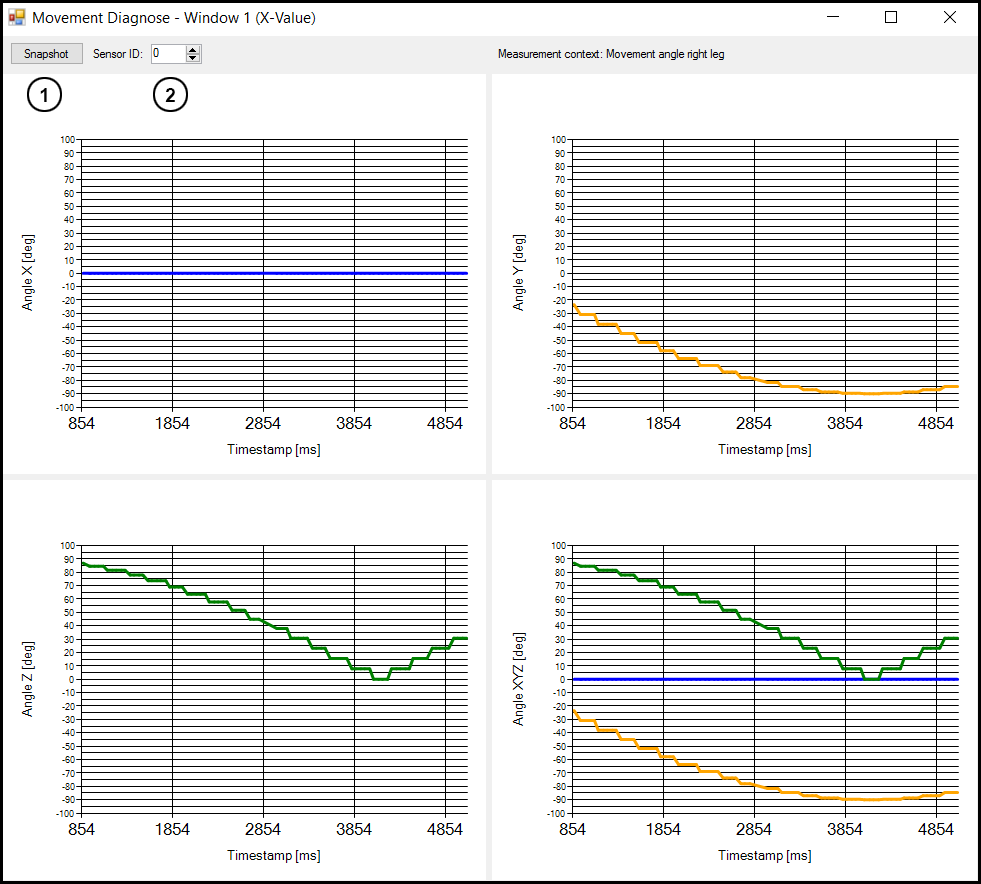
\includegraphics[width=1\linewidth]{03_Grafiken/Messsystem/ClientGraphDiagramm}
\caption[Diagramm Sensorwerte]{Diagramm der Sensorwerte}
\label{fig:clientgraphdiagramm}
\end{figure}




\subsection{Beschreibung HMI - Datenbank}
\label{kap:ClientGraphProgrammDatenbank}
W�hrend des Aufzeichnens von Sensorwerten erfolgt das Abspeichern in eine Datenbank. Diese beinhaltet die Daten f�r jeden Sensor einzeln mit den Beschleunigungswerten in x, y und z, sowie einen Zeitstempel. Die Datenbank kann durch das Bet�tigen des Buttons \textit{Show Database}, in der Hauptansicht des Programms, angezeigt werden (s. Abbildung \ref{fig:clientgraphdatabase}). Durch das Bet�tigen des Up-Down-Selectors erfolgt die Auswahl des entsprechenden Sensors.\\
Bei einer ernueten Messwertaufnahme wird der Datenbankinhalt gel�scht.

\begin{figure}[H]
\centering
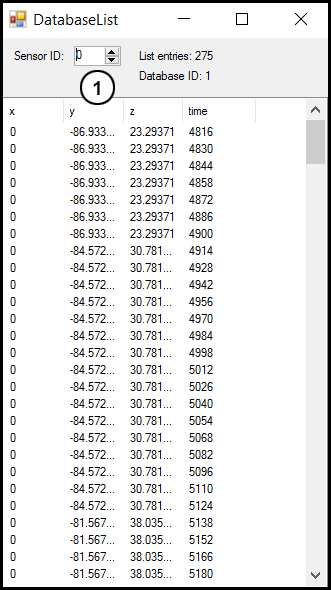
\includegraphics[width=0.5\linewidth]{03_Grafiken/Messsystem/ClientGraphDatabase}
\caption[Datenbank mit Sensorwerten]{Datenbank mit Sensorwerten}
\label{fig:clientgraphdatabase}
\end{figure}

\subsection{Beschreibung Programmaufbau}
\label{kap:ClientGraphCode}
In diesem Kapitel wird zu jeder Funktion (z.B. das Starten einer Messung) die dahinter liegenden Programm-Elemente aufgezeigt und erl�utert. Triviale Funktionalit�ten, wie z.B. das L�schen eines Textfeldes, werden dabei au�er Acht gelassen.

Die Elemente werden dabei mit der in der HMI angegebenen Bezeichnung beschrieben.

\begin{enumerate}
	%
	% Record to db
	%
	\item \textbf{Record to db}\\
	Das Starten einer Messwertaufnahme erfolgt durch das Bet�tigen des Buttons \textit{Record to db}. In der dazugeh�rigen Event-Routine (s. Listing \ref{lst:recordToDb} Zeile 1-19) erfolgt zun�chst eine Abfrage der Button-Beschriftung (Zeile 3), da nur ein Element zum Stoppen / Starten einer Messwertaufnahme genutzt wird. In dieser Abfrage wird ein Dialog eingeblendet, der das L�schen des bisherigen Datenbankinhaltes veranlasst (Zeile 5-9). \\
	Das L�schen der Datenbank erfolgt innerhalb eines Background-Tasks (s. Zeile 23-32). Hierbei wird in Zeile 26 und 27 die Datenbank 1 und 2 mit den entsprechenden Connectionstrings gel�scht. In Zeile 28 und 29 erfolgt das Erstellen der neuen Datens�tze f�r Datenbank 1 und 2. Zeile 30 gibt den Datensatz 1 an die Routine \textit{x\_RunWOrkerCompleted()} weiter. In dieser Routine wird die boolsche Variable \textit{recordIsActive} gesetzt, sodass in der Event-Routine \textit{tcpMsgRecEvent()}, die beim Eintreffen eines Messwerts aufgerufen wird, Werte in die Datenbank geschrieben werden k�nnen. Sobald die Variable wieder zur�ckgesetzt ist, erfolgt kein weiteres Schreiben in die Datenbank.
	\input{02_Inhalt/Messsystem/Listings/recordToDb}
	%
	% Export db to txt
	%
	\item \textbf{Export db to txt file}\\
	Das Exportieren der gespeicherten Messwerte (Formatierung: CSV-Datei, Trennzeichen: Semikolon) erfolgt durch das Bet�tigen des Buttons \textit{Export db to txt}. In der dazugeh�rigen Event-Routine wird dazu ein Background-Task gestartet \ref{lst:exportDb} Zeile 1-16). In dieser Routine wird zun�chst die maximale Zeilenanzahl, sowie die �berschrift f�r das Textdokument gesetzt.\\
	In Zeile 7-15 erfolgt das Schreiben der Daten in eine Textdatei. Diesbez�glich wird f�r jeden Sensor eine seperate Datei mit spezifischen DAteinamen erstellt. Das Setzen des Dateinamens erfolgt im Textfeld \textit{Context} innerhalb der Main-Gui. Wird kein Name angegeben, so tragen die Dateien die Bezeichnung \textit{noname\_x.txt}. \\
	Da w�hrend des Schreibvorgangs alle Buttons deaktiviert werden, erfolgt in der Routine \textit{...RunWorkerCompleted()} das Re-Aktivieren der entsprechenden Elemente.
	\input{02_Inhalt/Messsystem/Listings/exportDb}
	%
	% Import extracted steps
	%
	\item \textbf{Upload steps}\\
	Zun�chst muss in das Textfeld \textit{db name} die Bezeichnung der Tabelle eingegeben werden, in die etwas importiert werden soll (Tabellenname in der externen SQL-Datenbank - s. Beschreibung Kapitel \ref{kap:DatabaseLayout}).
	Durch das Bet�tigen des Buttons erscheint dann ein Dialog, in dem der Bediener eine CSV-Datei (ohne �berschrift) ausw�hlen muss. Diese Textdatei muss folgendes Format des Dateinamens aufweisen: tableX.txt (X steht f�r die Zahl des Sensors, z.B. 0, 1, 2, etc.).\\
	Anschlie�end erfolgt das Hochladen in eine externe SQL-Datenbank.
	In einer sp�teren Version wird es nur noch einen Button geben, mit dem die Schrittfolge automatisch extrahiert und in die externe Datenban k hochgeladen wird.
	\input{02_Inhalt/Messsystem/Listings/uploadSteps}
	%
	% Calibrate Sensors
	%
	\item \textbf{Calibrate Sensors}\\
	Das Starten der Kalibrierung erfolgt durch das Bet�tigen des Buttons \textit{Calibrate Sensors}. In der dazugeh�rigen Event-Routine (s. Listing \ref{lst:calibrateSensor} Zeile 1-9) werden zun�chst die Kalibrierwerte (Zeile 5), sowie der Merker, f�r das Durchf�hren einer Kalibrierung (Zeile 6), zur�ckgesetzt.\\
	In Zeile 8 wird der Button deaktiviert und erst wieder aktiviert wenn die Kalibrierung abgeschlossen ist.\\
	Das Ausf�hren der Kalibrierung erfolgt in der Event-Routine \textit{tcpMsgRecEvent()} (Zeile 11-52), die beim Eintreffen eines Messwerts ausgef�hrt wird. Ist der Button \textit{Calibrate Sensors} deaktiviert und der Merker f�r die durchgef�hrte Kalibrierung \textit{sensorCalibrationSet[]} gesetzt erfolgt das Kalibrieren in den Zeilen 18-36. Dabei wird zu Beginn in den Zeilen 18-20 der Quadrant gepr�ft, in dem sich das \gls{KS} des Sensors befindet. Demnach erfolgt ein Abbruch, wenn ein Sensor sich nicht innerhalb der zul�ssigen Quadranten (s. Abbildung \ref{fig:ZulQuadranten}) befindet.
	
	\begin{figure}[h]
	\centering
	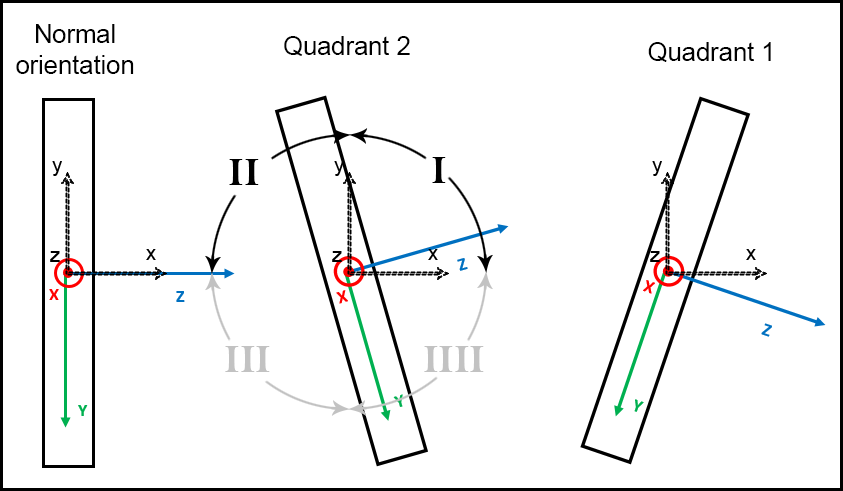
\includegraphics[width=0.7\linewidth]{03_Grafiken/Messsystem/Quadranten}
	\caption[Zul�ssige Quadranten]{Zul�ssige Quadranten}
	\label{fig:ZulQuadranten}
	\end{figure}

	\input{02_Inhalt/Messsystem/Listings/calibrateSensor}
	%
	% Show graph
	%
	\item \textbf{Show graph}\\
	Das Visualisieren der Messwerte erfolgt innerhalb eines Hintergrund-Tasks. Diesbez�glich wird der Graph aktualisiert, sobald ein neuer Messwert empfangen wurde. Beim Empfangen eines Messwerts erfolgt der Aufruf der Event-Routine \textit{tcpMsgRecEvent()} (s. Listing \ref{lst:showGraph} Zeile 1-4). Innerhalb dieser Routine wird gepr�ft, ob die Checkbox zum Anzeigen der Visualisierung gesetzt und ob die Windows Form bereits deklariert ist. Ist dies der Fall, so erfolgt die �bergabe aller Messwerte, sowie der Sensor-ID an die Routine \textit{setNewChartData()} (s. Zeile 3).\\
	In dieser Routine wird zun�chst gepr�ft, ob die ausgew�hlte ID (mit dem Up- Down-Selector) mit der �bertragenen Sensor-ID �bereinstimmt. Ist dies der Fall so erfolgt das Setzen eines Events \textit{chartData()} (s. Zeile 8). In der Event-Routine \textit{OnChartEvent()} wird zun�chst gepr�ft, ob die darzustellenden Daten bereits in dem Daten-Array vorhanden sind (Pr�fen gegen Vorinitialisierung -9999). Ist dies der Fall so wird die Routine \textit{setDataToGraph()} aufgerufen (�bergabewert: Sensordaten). In dieser Routine ist das Visualisieren der Messwerte implementiert (s. Zeile 16-24). Dargestellt ist der Code f�r das Setzen der Sensorwerte auf die X-Achse. Zeile 18-19 zeigt das Setzen der Achsbeschriftung und Zeile 21-22 zeigt das Setzen eines Messpunkts.
	\input{02_Inhalt/Messsystem/Listings/showGraph}
	%
	% Show database
	%
	\item \textbf{Show database}\\
	Das Darstellen der Datenbank, indem sich die aufgezeichneten Messwerte befinden, erfolgt durch das Setzen der entsprechenden Checkbox. Das Pr�fen, ob die Checkbox gesetzt ist erfolgt inerhalb der verbundenen Event-Routine (s. Listing \ref{lst:showDb} Zeile 4). Entsprechend der Datenbank-ID wird die Datenbank ausgew�hlt und eine Liste mit dessen Inhalt erzeugt (s. Zeile 6) und dargestellt (s. Zeile 7).
	\input{02_Inhalt/Messsystem/Listings/showDb}
\end{enumerate}



	\chapter{Datenbank Layout}
\label{kap:DatabaseLayout}
Es existieren insgesamt zwei Systeme (Mess- und Robotersystem), von denen jedes �ber eine lokale Datenbank verf�gt. Dar�ber hinaus exisitert eine externe, �ber das Internet erreichbare Cloud, in der die gesamten Bewegungsdaten f�r den Roboter hinterlegt sind (s. Abbildung \ref{fig:dblayout}). Diese sind als Integer-Werte abgelegt und mit dem Faktor 100 multipliziert, sodass diese Daten vom Prinzip unmodifziert sind und ein breites Anwedungsgebiet erm�glichen. Das Konvertieren in die nutzbaren Stellgr��en f�r das entsprechende System (in diesem Fall das Robotersystem) erfolgt lokal.

\begin{figure}[H]
\centering
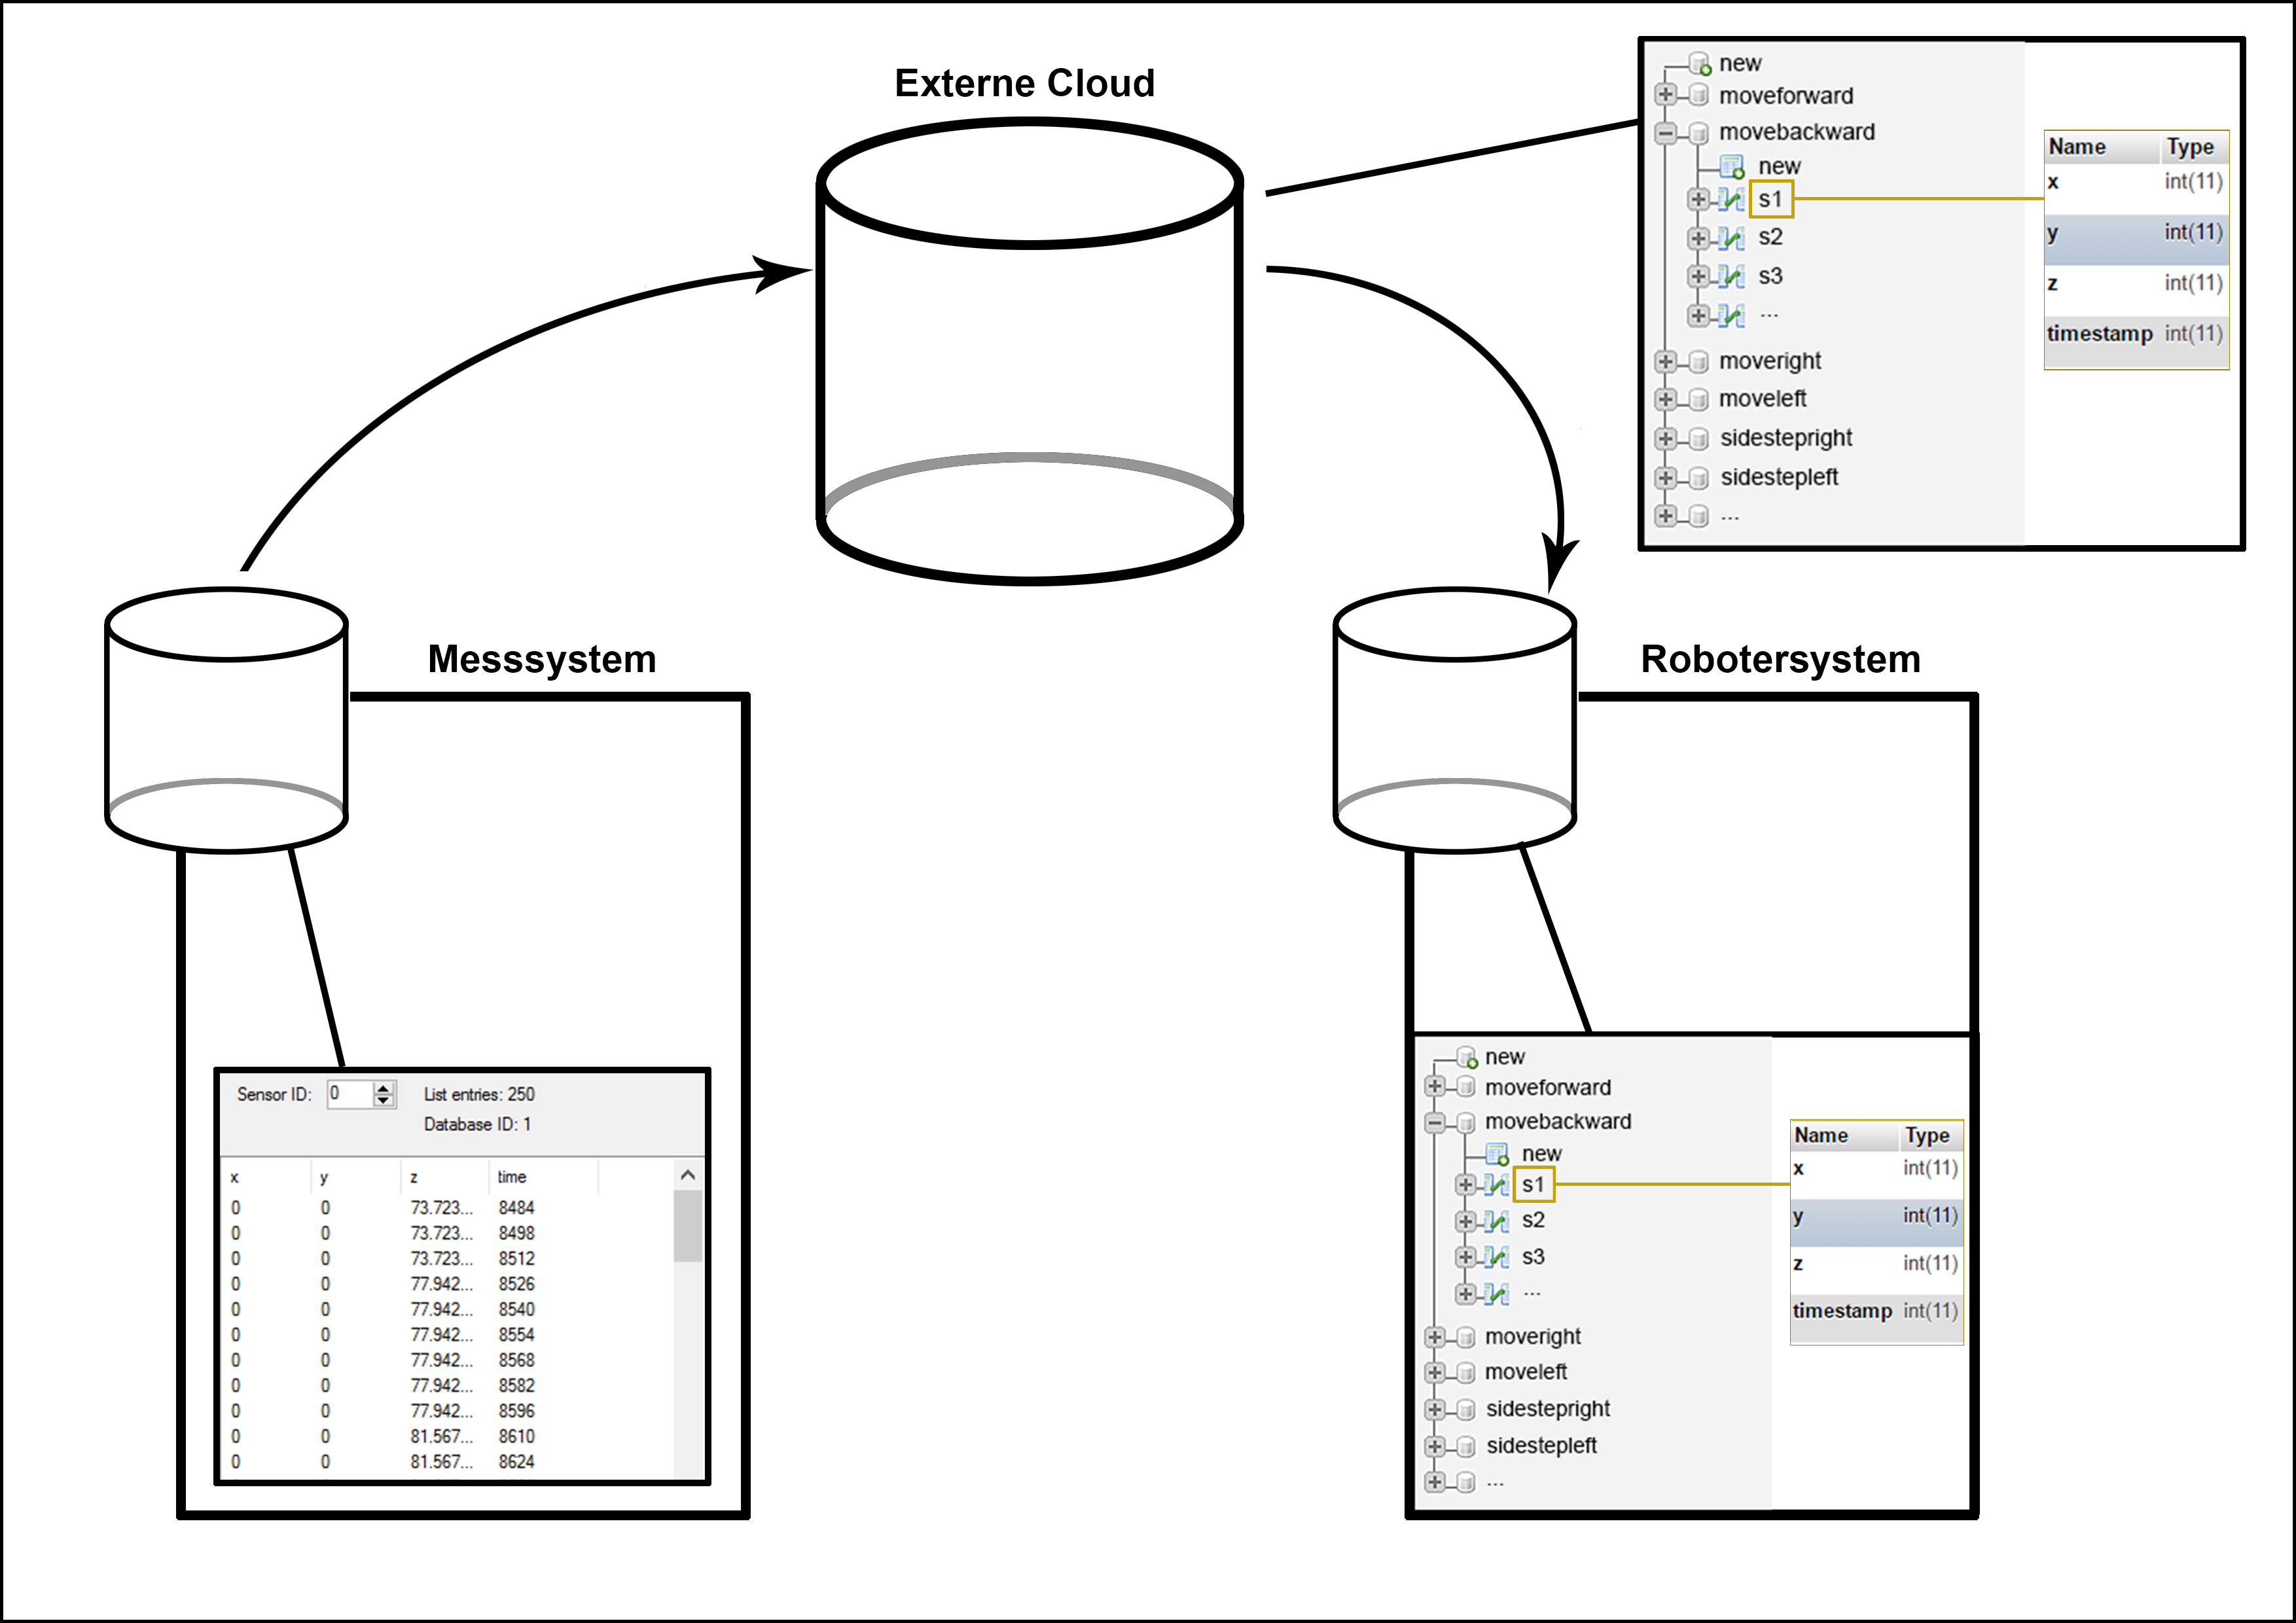
\includegraphics[width=1.0\linewidth]{03_Grafiken/DatabaseLayout/dblayout}
\caption[Layout der Datenbanken]{Layout der Datenbanken}
\label{fig:dblayout}
\end{figure}

Der oben dargestellte zylinderf�rmige Komponente repr�sentiert die externe Cloud, welche �ber das Internet erreichbar ist. Diese beinhaltet die Bewegungsdaten f�r alle Motoren, welche zuvor durch das Messsystem aufgenommen und extrahiert wurden. Die Struktur (s. seitlicher Bereich) besteht aus mehreren Datenbanken, von denen jede mehrere Tabellen enth�lt, in denen die Sensorwerte hinterlegt sind. Abbildung \ref{fig:cloudcontent} zeigt exemplarisch den Aufbau der Cloud.

\begin{figure}[H]
\centering
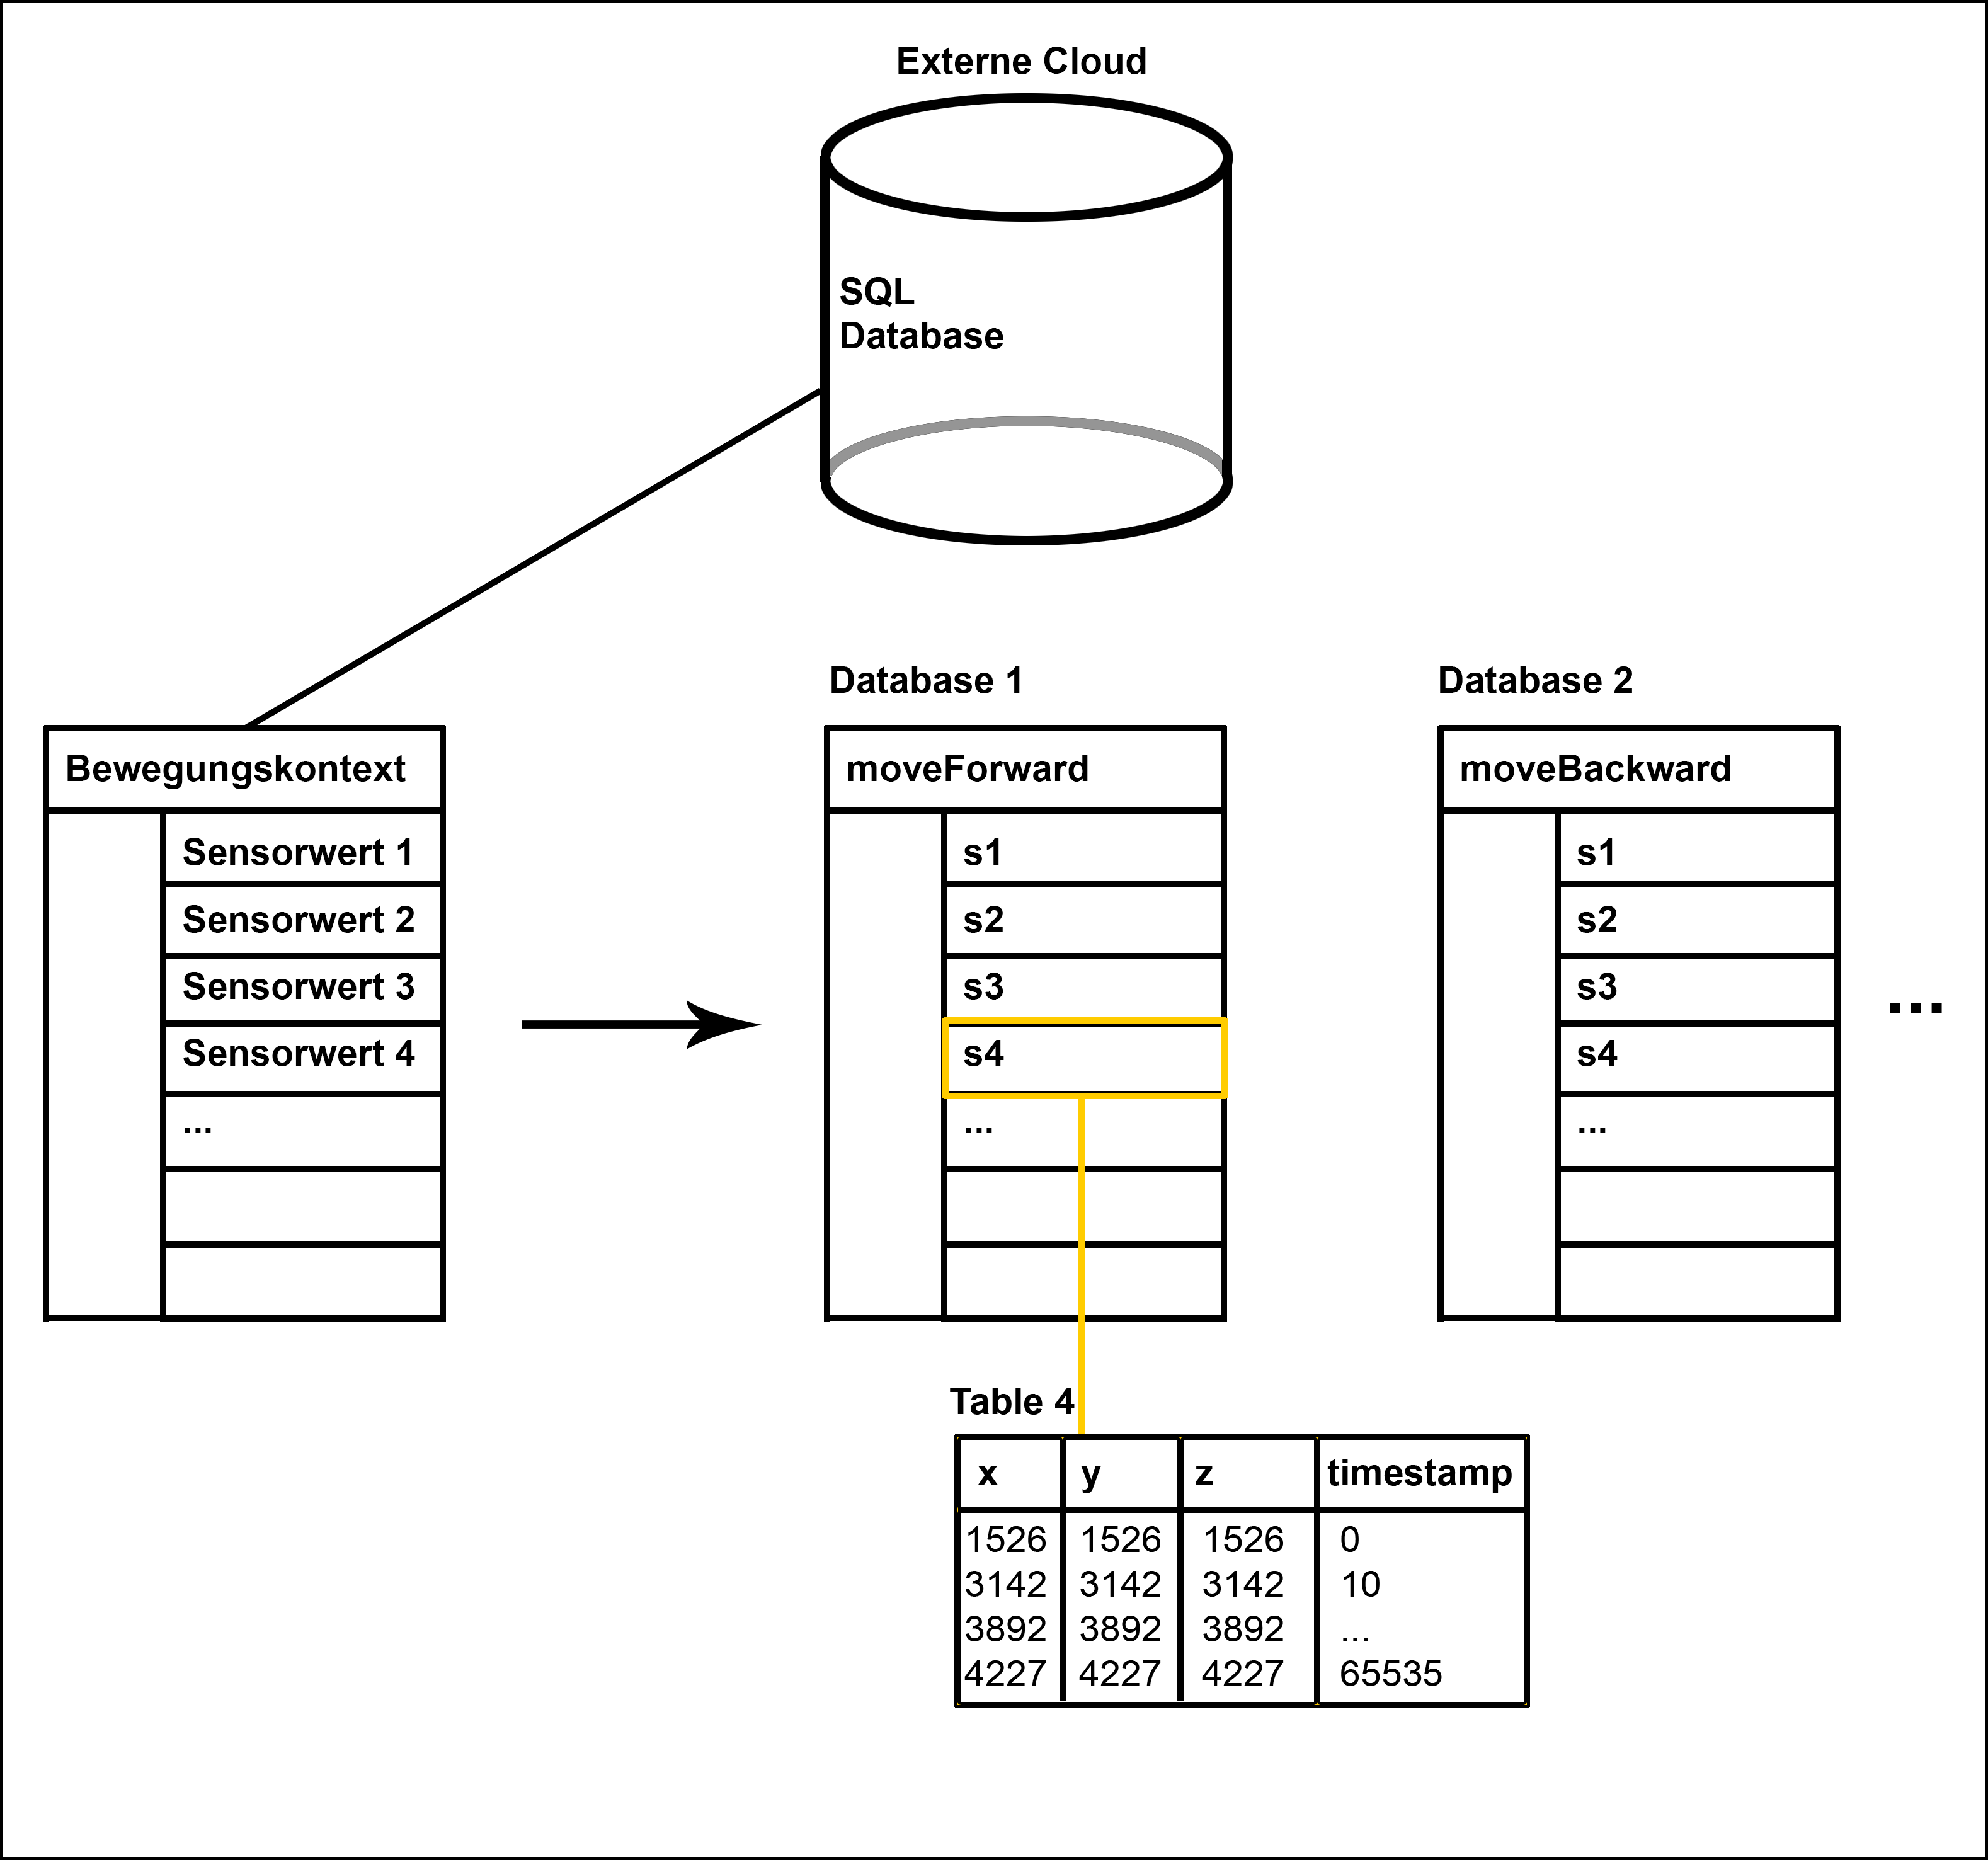
\includegraphics[width=1.0\linewidth]{03_Grafiken/DatabaseLayout/CloudContent}
\caption[Struktur der externen Cloud]{Struktur der externen Cloud}
\label{fig:cloudcontent}
\end{figure}

Die links dargestellte Komponente zeigt den grunds�tzlichen Aufbau einer Datenbank mit den darin liegenden Tabellen. Darin enthalten sind die Werte aller Sensoren in extrahierter Form, multipliziert mit dem Faktor 100. Die beiden rechts dargestellten Tabellen zeigen beispielhaft den Kontext der Datenbanken. Dieser ist mit der entsprechenden Bewegungsart definiert (z.B. Vorw�rtsgehen, R�ckw�rtsgehen, etc.). Unterhalb der beiden Tabellen wird der Inhalt einer Tabelle innerhalb einer Datenbank (z.B. Tabelle \textit{s4} in der Datenbank \textit{moveForward}) aufgezeigt. Dabei ist zu beachten, dass die Eintr�ge aus maximal 2 byte bestehen d�rfen, da das Protokoll mehr nicht zul�sst (s. Kapitel \ref{kap:Protokoll}). F�r die Sensorwerte ist dies irrelevant, da diese max. $ \alpha = 90 [deg]$, bzw. 9000 erreichen k�nnen. Wichtig ist dies allerdings f�r den Zeitstempel. Dieser kann max. 65535 erreichen, was eine Messdauer von ca. $ \Delta t = 60 [s]$ entspricht. F�r die grunds�tzliche Fortbewegung ist es ausreichend, f�r ganze Bewegungstasks (z.B. geskriptes Inlineskaten) jedoch nicht.


	\chapter{Robotersystem}
\label{kap:Robotersystem}
Das Robotersystem beschreibt das Endprodukt dieses Projekts - eine mechanische Einheit mit bipedaler Fortbewegung. Diesbez�glich ist zu beachten, dass keinerlei Autonomie und Intelligenz in dem System steckt. Der Schwerpunkt liegt einzig auf der datenbankbasierten Fortbewegung. \\
Um eine bestm�gliche Bewegungsfreiheit zu gew�hrleisten, muss das mechanische System perfekt mit dem des Menschen �bereinstimmen. Nur dann sind dem Aufzeichnen, sowie dem Konvertieren in Bewegungsfolgen keine Grenzen gesetzt.\\
In diesem Projekt wird das Robotersystem mit manueller Eingabe bewegt (gesteuert). Die entsprechenden Softwarekomponenten sind diesbez�glich im Kapitel \ref{kap:Softwarekomponenten} beschrieben.\\
Das mechanische Modell findet im Kapitel \ref{kap:MechModell} Erl�uterung.

\section{Ansteuerung}
\label{kap:Ansteuerung}
Der Aufbau des Gesamtsystem und dessen Funktionsweise ist in Abbildung XXX prinzipiell dargestellt.

\begin{figure}[H]
\centering
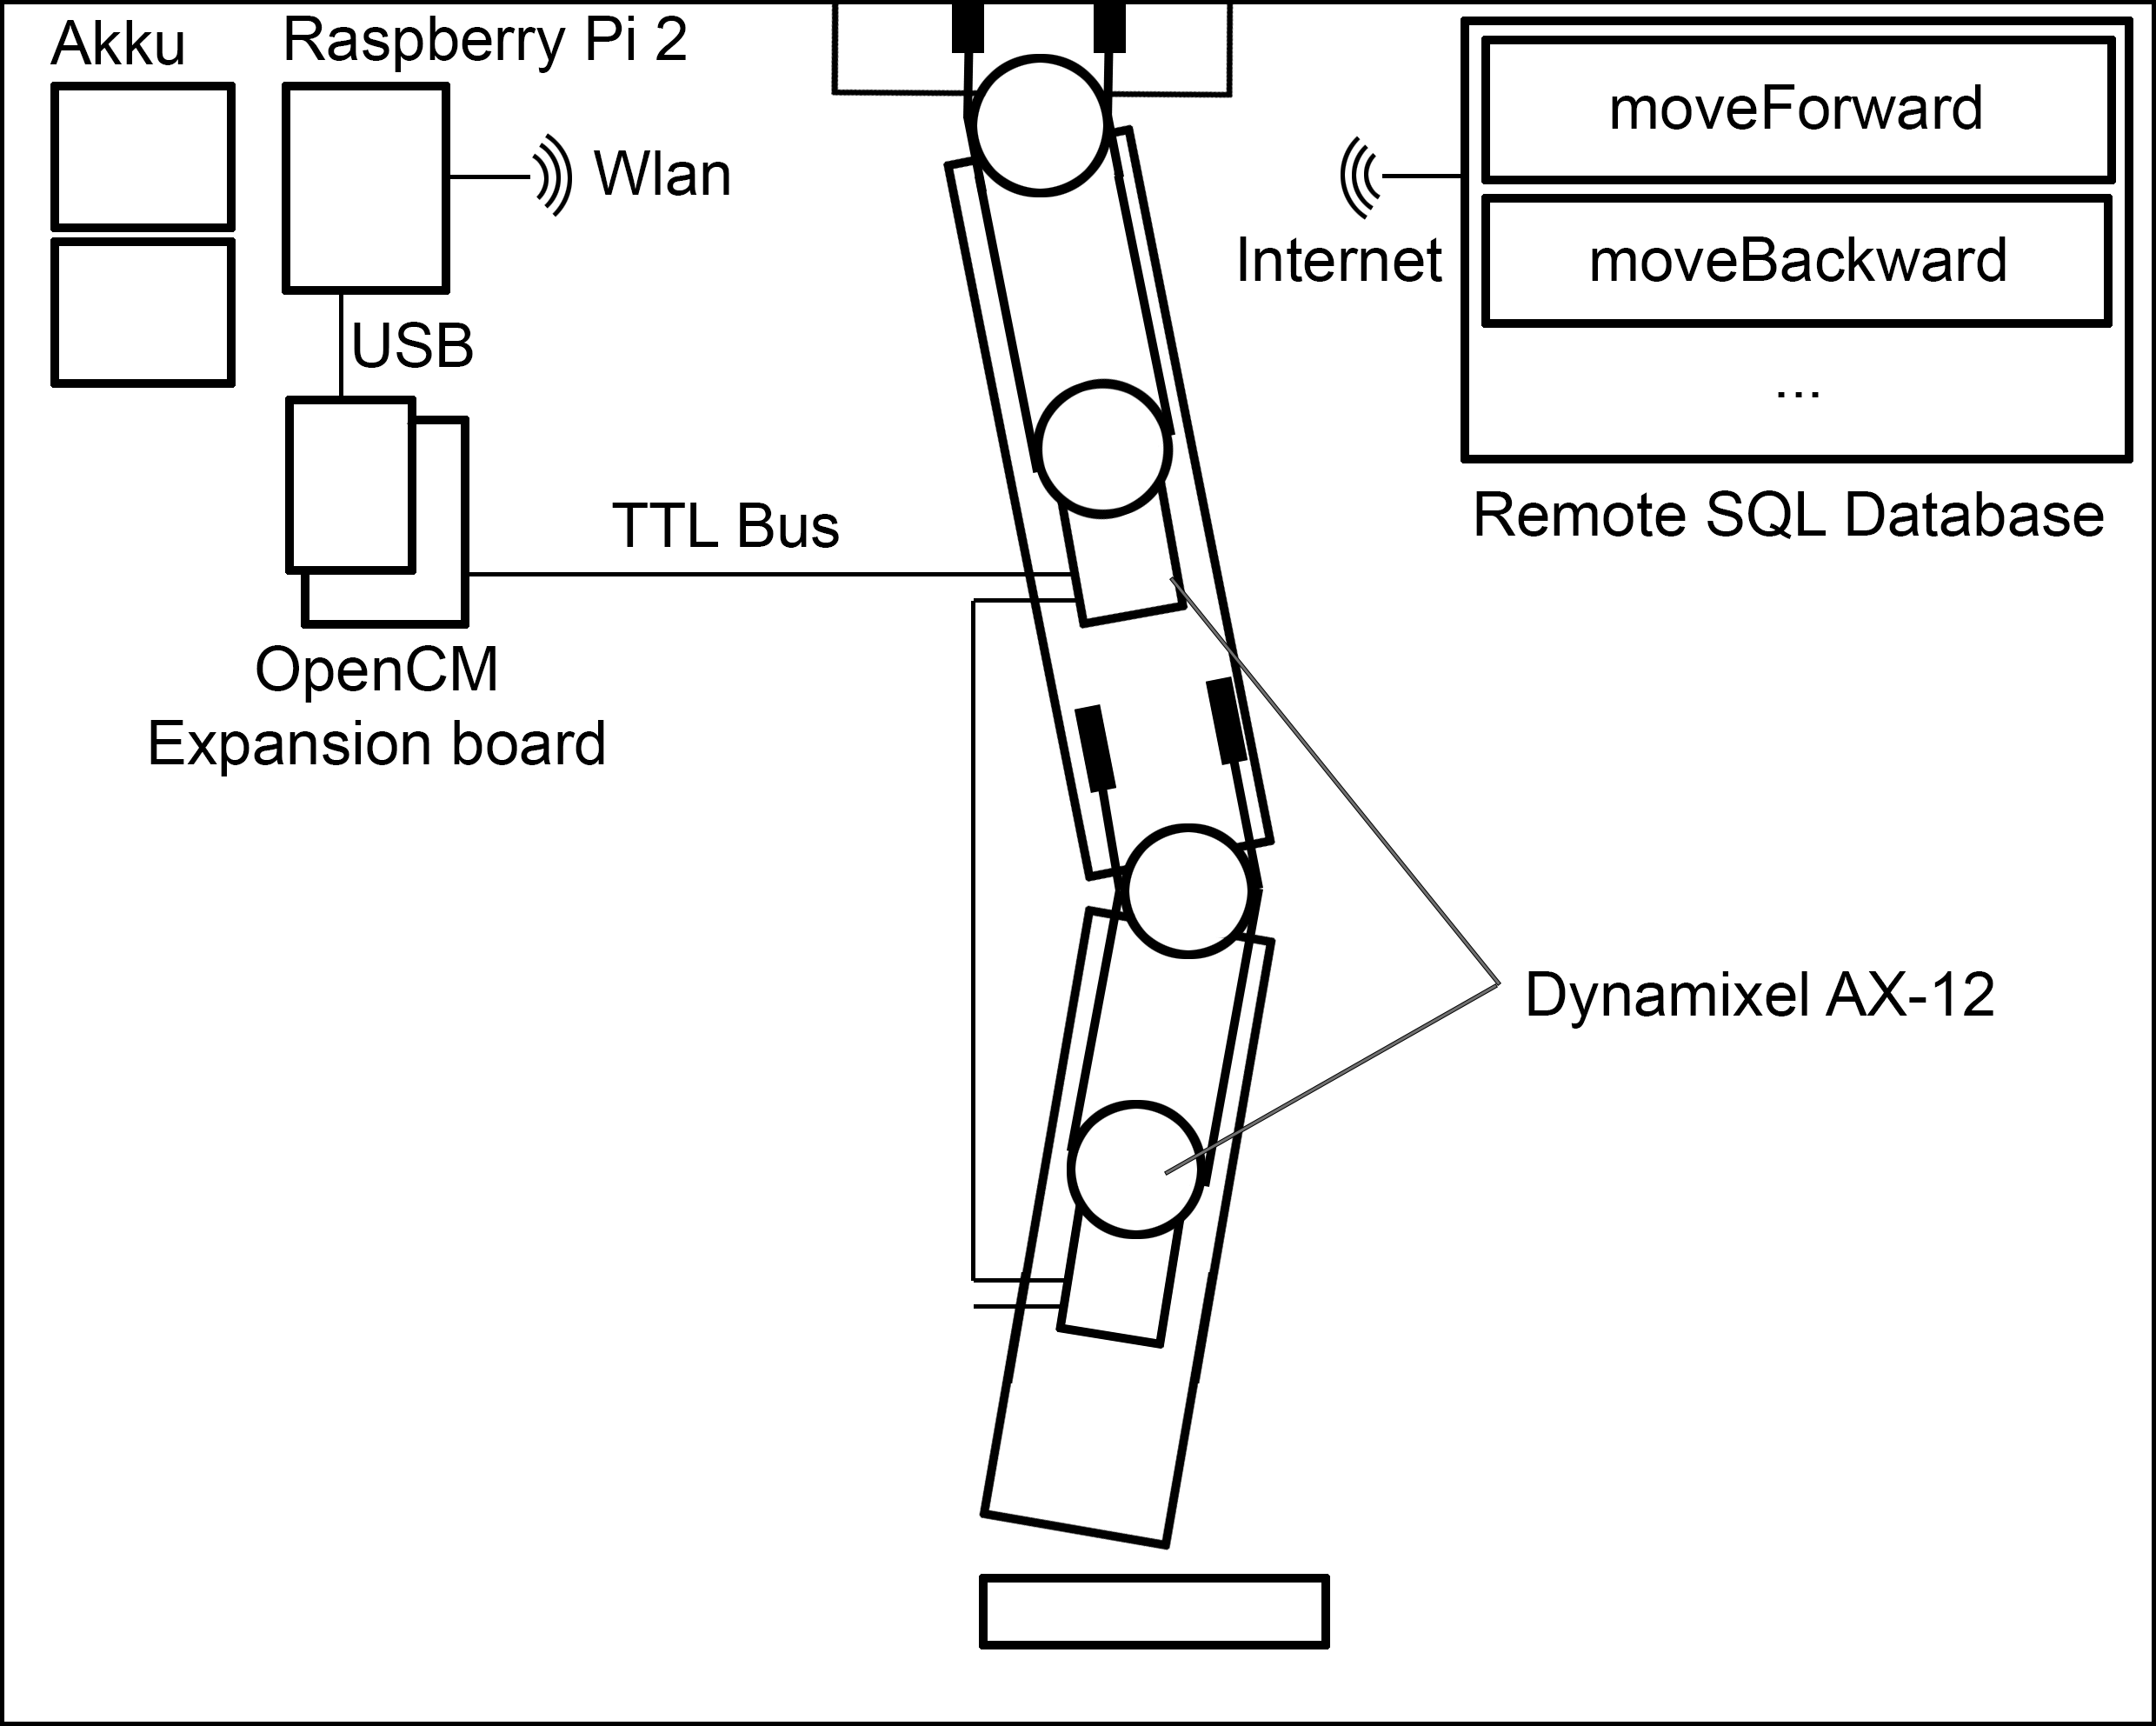
\includegraphics[width=1.0\linewidth]{03_Grafiken/Robotersystem/Aufbau}
\caption[Ansteuerung / Aufbau (Prinzip)]{Ansteuerung / Aufbau (Prinzip)}
\label{fig:aufbau}
\end{figure}

Dabei ist zun�chst das mechanische Modell vernachl�ssigbar, da dieses im weiteren Verlauf Erl�uterung findet. Zun�chst wird die softwaretechnische Seite betrachtet und dessen elektronischen Komponenten, die zur Ansteuerung des Gesamtsystems genutzt werden, erl�utert.\\
Diesbez�glich befindet sich im oberen linken Teil der GRafik die Konstellation der beteiligten Baugruppen und deren Verkn�pfung zueinander. Der Raspberry Pi 2 dient als Steuerzentrale, auf dem das \gls{BS} Windows 10 IOT installiert ist. Darauf ist eine Software aktiv, mit der die gesamte Reglung des Systems abgearbeitet wird. Entsprechend erfolgt das Senden von Befehlen (zur Ansteuerung der Motoren) vom Raspberry Pi aus �ber eine USB-Schnittstelle hin zum OpenCM Board. Dieses Board liest die Befehle und gibt diese an die Motoren (Dynamixel AX-12) weiter. Das Expansion Board ist notwendig, da das OpenCM-Board keine TTL-Schnittstelle zur Verf�gung stellt.\\
Der eigentlich Clou des Systems besteht darin, dass beim Neustart (sofern notwendig) die Bewegungss�tze von einer externen Datenbank heruntergeladen werden. Diesbez�glich verf�gt der Raspberry Pi �ber eine Wlan, bzw. UMTS-Schnittstelle. Die SQL-Datenbank ist �ber das Internet erreichbar, sodass stets aktuelle Bewegungss�tze zur Verf�gung stehen. Die BEwegungss�tze werden mit dem, in Kapitel \ref{kap:Messsystem} beschriebenen Messsystem erstellt / erweitert.
\subsection{Protokoll}
% Sequentielle Block�bertragung f�r max 8 Motoren

\subsection{Testprogramm}
% WriteToComPort

\subsection{Kontrollprogramm}
% MovementControl

\subsection{Clientprogramm}
% Programm auf dem OpenCM
\section{Mechanisches Modell}
\label{kap:MechModell}

\subsection{Prinzipieller Aufbau}


	\noindent
\begin{minipage}{\textwidth}
\chapter{Zusammenfassung}
\label{sec:Zusammenfassung}
Zun�chst soll ein �berblick gegeben werden, der die wichtigsten Aspekte des gesamten Systems beschreibt (s. Tabell \ref{tab:AspekteGesamtsystem}).

\begin{center}
\begin{tabular}{|p{5cm}|p{3cm}|p{3cm}|}
	\hline 
	\textbf{Beschreibung} & \textbf{Kontext} & \textbf{Begr�ndung} \\ 
	\hline 
	Es k�nnen max. 8 Motoren per Zyklus angesprochen werden & Ansteuerung Robotersystem & Probleme Zusammensetzen mehrerer Bytes \\ 
	\hline 
	Die Datenbankgr��e darf f�r den Zeitstempel max. 65535 (2 byte) aufweisen & Ansteuerung Robotersystem & Aktuelle Implementierung Protokoll \\ 
	\hline 
	Das System l�sst nur das aktive Steuern zu. Autonomie ist nicht gegeben. &  Ansteuerung Robotersystem & Funktionsumfang aktueller Version \\ 
	\hline 
	&  &  \\ 
	\hline 
\end{tabular} 
\end{center}

Da eine k�nstliche Intelligenz zu unvorhersehbaren, gef�hrlichen Situationen f�hren kann, muss ein, dem Menschen �hnlich dynamisches System, in seiner Freiheit beschr�nkt werden. Der Begriff Freiheit definiert in diesem Kontext das eigenst�ndige Lernen ohne menschliche Kontrolle. \\
Ein datenbankbasiertes System besitzt hingegen nur die F�higkeiten, welche in der Datenbank hinterlegt sind. Dies bringt den Vorteil der Berechenbarkeit mit sich.
\vspace{2.5cm}
\chapter{Ausblick}
\label{sec:Ausblick}
 Stark unausgereift hingegen ist das zusammenh�ngende Verarbeiten visueller Eindr�cke, auditiver Wahrnehmungen, sowie vestibul�ren Werten und sensomotorischen F�higkeiten.
\end{minipage}

	
	\pagenumbering{Roman}	% R�mische Seitenzahlen (IV)
	\bibliography{02_Inhalt/Literatur}
	\appendix 
\refstepcounter{chapter}
%
% Usability-Test
%
%\section{Usability-Test} 
\label{app:Usability}
\subsection{Ablauf, Beschreibung, Evaluationsbogen}
% ------------------------------
% Bild Usability Beschreibung
% ------------------------------
\begin{figure}[H]
	\centering
		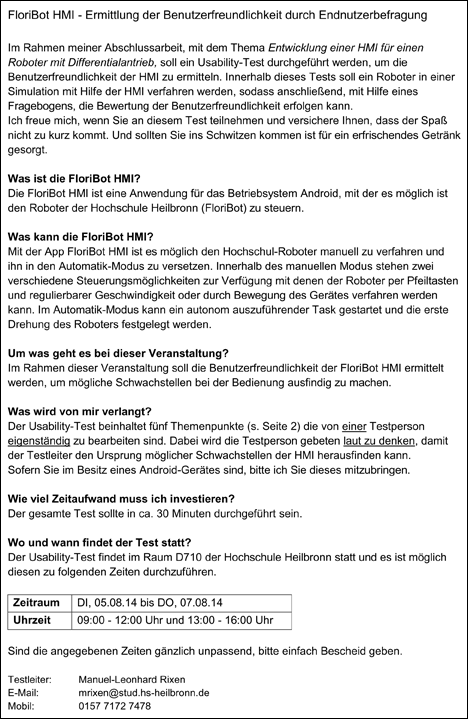
\includegraphics[width=0.85\textwidth]{03_Grafiken/Anhang/UsabilityBogen/UsabilityBeschreibung.png}
	\caption[Beschreibung des Usability-Tests]{Beschreibung des Usability-Tests}
	\label{fig:UsabilityBeschreibung}
\end{figure}
% ------------------------------
% Bild Usability Ablauf
% ------------------------------
\begin{figure}[H]
	\centering
		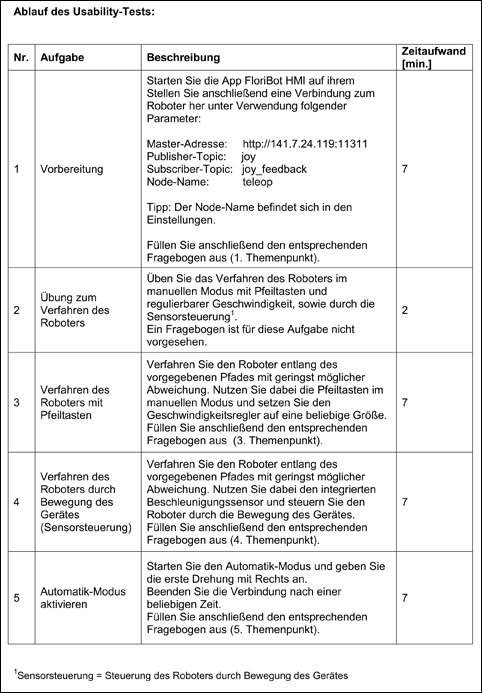
\includegraphics[width=0.85\textwidth]{03_Grafiken/Anhang/UsabilityBogen/UsabilityAblauf.png}
	\caption[Ablauf des Usability-Tests]{Ablauf des Usability-Tests}
	\label{fig:UsabilityAblauf}
\end{figure}
% ------------------------------
% Bilder des Usability Evaluationsbogens
% ------------------------------
\begin{figure}[H]
	\centering
		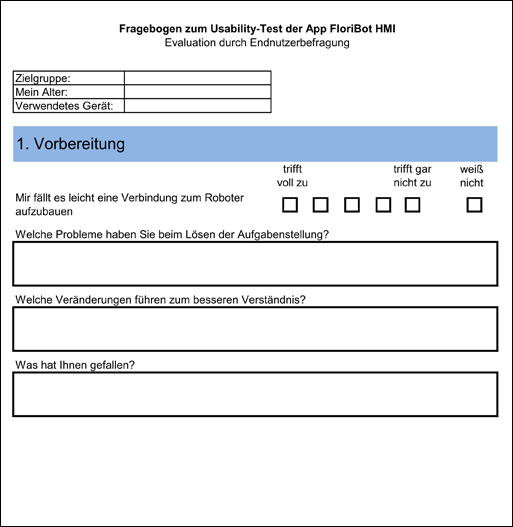
\includegraphics[width=0.85\textwidth]{03_Grafiken/Anhang/UsabilityBogen/UsabilityEvaluationsbogen.png}
	\caption[Evaluationsbogen des Usability-Tests - Seite 1]{Evaluationsbogen des Usability-Tests - Seite 1}
	\label{fig:UsabilityEvaluationsbogen}
\end{figure}
\newpage
\begin{figure}[H]
	\centering
		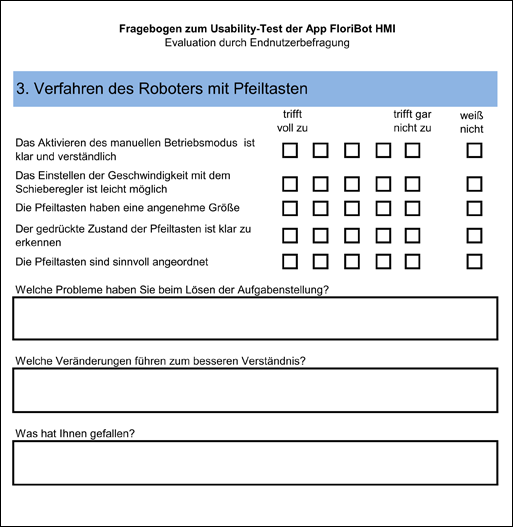
\includegraphics[width=0.85\textwidth]{03_Grafiken/Anhang/UsabilityBogen/UsabilityEvaluationsbogen1.png}
	\caption[Evaluationsbogen des Usability-Tests - Seite 2]{Evaluationsbogen des Usability-Tests - Seite 2}
	\label{fig:UsabilityEvaluationsbogen}
\end{figure}
\newpage
\begin{figure}[H]
	\centering
		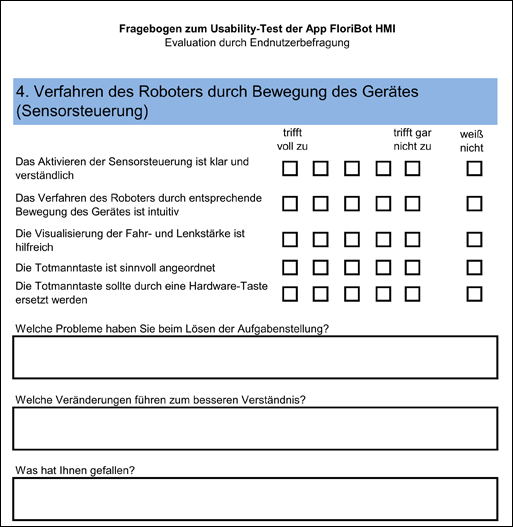
\includegraphics[width=0.85\textwidth]{03_Grafiken/Anhang/UsabilityBogen/UsabilityEvaluationsbogen2.png}
	\caption[Evaluationsbogen des Usability-Tests - Seite 3]{Evaluationsbogen des Usability-Tests - Seite 3}
	\label{fig:UsabilityEvaluationsbogen}
\end{figure}
\newpage
\begin{figure}[H]
	\centering
		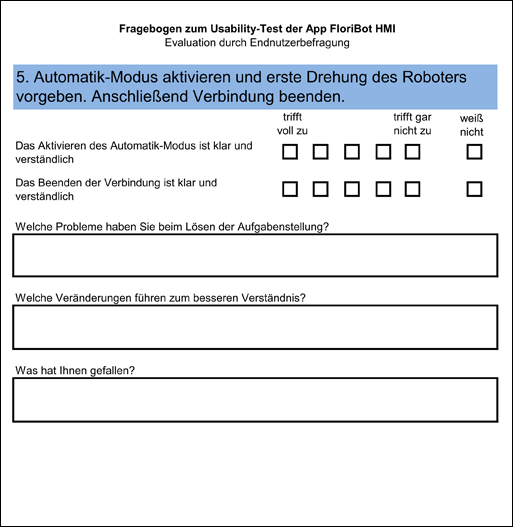
\includegraphics[width=0.85\textwidth]{03_Grafiken/Anhang/UsabilityBogen/UsabilityEvaluationsbogen3.png}
	\caption[Evaluationsbogen des Usability-Tests - Seite 4]{Evaluationsbogen des Usability-Tests - Seite 4}
	\label{fig:UsabilityEvaluationsbogen}
\end{figure}
\newpage
\begin{figure}[H]
	\centering
		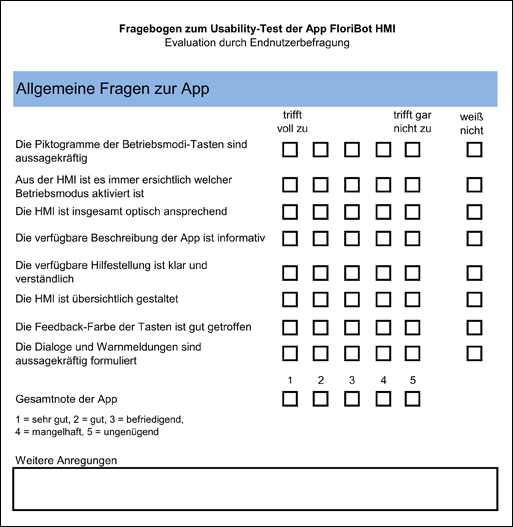
\includegraphics[width=0.85\textwidth]{03_Grafiken/Anhang/UsabilityBogen/UsabilityEvaluationsbogen4.png}
	\caption[Evaluationsbogen des Usability-Tests - Seite 5]{Evaluationsbogen des Usability-Tests - Seite 5}
	\label{fig:UsabilityEvaluationsbogen}
\end{figure}
\newpage
\newpage
\subsection{Diagramme}
\label{app:UsabilityKreisdiagramme}
% ------------------------------
% Aufgabenteil 3 - Aussage 1
% ------------------------------
\begin{figure}[H]
	\centering
		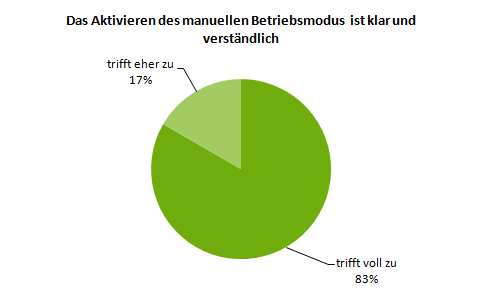
\includegraphics[width=0.85\textwidth]{03_Grafiken/Anhang/UsabilityDiagramme/Aufgabenteil3Aussage1.png}
	\caption[Diagramm zum Analysieren der Benutzerfreundlichkeit beim Verfahren mit Pfeiltasten - Aussage 1]{Diagramm zum Analysieren der Benutzerfreundlichkeit beim Verfahren mit Pfeiltasten - Aussage 1}
	\label{fig:Aufgabenteil3Aussage1}
\end{figure}
% ------------------------------
% Aufgabenteil 3 - Aussage 2
% ------------------------------
\begin{figure}[H]
	\centering
		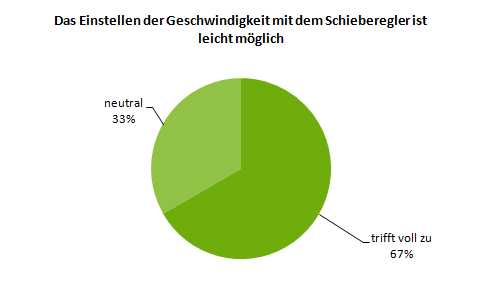
\includegraphics[width=0.85\textwidth]{03_Grafiken/Anhang/UsabilityDiagramme/Aufgabenteil3Aussage2.png}
	\caption[Diagramm zum Analysieren der Benutzerfreundlichkeit beim Verfahren mit Pfeiltasten - Aussage 2]{Diagramm zum Analysieren der Benutzerfreundlichkeit beim Verfahren mit Pfeiltasten - Aussage 2}
	\label{fig:Aufgabenteil3Aussage2}
\end{figure}
% ------------------------------
% Aufgabenteil 3 - Aussage 3
% ------------------------------
\begin{figure}[H]
	\centering
		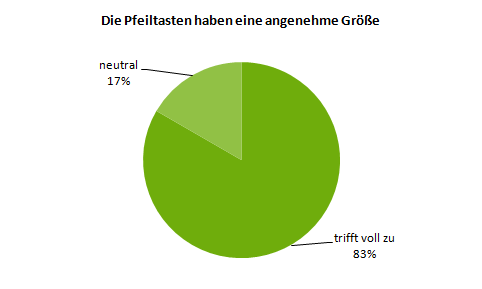
\includegraphics[width=0.85\textwidth]{03_Grafiken/Anhang/UsabilityDiagramme/Aufgabenteil3Aussage3.png}
	\caption[Diagramm zum Analysieren der Benutzerfreundlichkeit beim Verfahren mit Pfeiltasten - Aussage 3]{Diagramm zum Analysieren der Benutzerfreundlichkeit beim Verfahren mit Pfeiltasten - Aussage 3}
	\label{fig:Aufgabenteil3Aussage3}
\end{figure}
% ------------------------------
% Aufgabenteil 3 - Aussage 4
% ------------------------------
\begin{figure}[H]
	\centering
		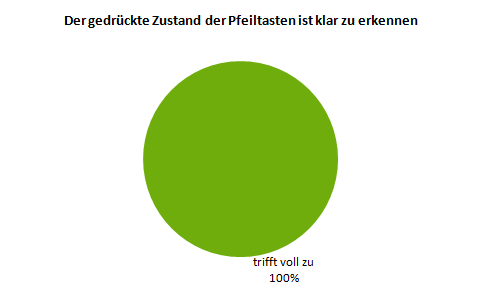
\includegraphics[width=0.85\textwidth]{03_Grafiken/Anhang/UsabilityDiagramme/Aufgabenteil3Aussage4.png}
	\caption[Diagramm zum Analysieren der Benutzerfreundlichkeit beim Verfahren mit Pfeiltasten - Aussage 4]{Diagramm zum Analysieren der Benutzerfreundlichkeit beim Verfahren mit Pfeiltasten - Aussage 4}
	\label{fig:Aufgabenteil3Aussage4}
\end{figure}
% ------------------------------
% Aufgabenteil 3 - Aussage 5
% ------------------------------
\begin{figure}[H]
	\centering
		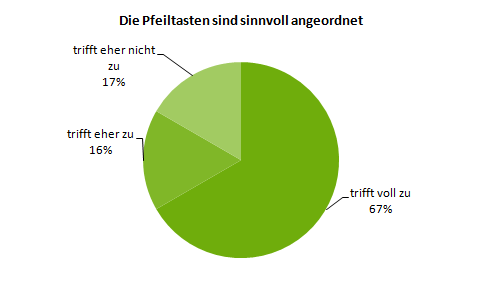
\includegraphics[width=0.85\textwidth]{03_Grafiken/Anhang/UsabilityDiagramme/Aufgabenteil3Aussage5.png}
	\caption[Diagramm zum Analysieren der Benutzerfreundlichkeit beim Verfahren mit Pfeiltasten - Aussage 5]{Diagramm zum Analysieren der Benutzerfreundlichkeit beim Verfahren mit Pfeiltasten - Aussage 5}
	\label{fig:Aufgabenteil3Aussage5}
\end{figure}
% ------------------------------
% Aufgabenteil 4 - Aussage 1
% ------------------------------
\begin{figure}[H]
	\centering
		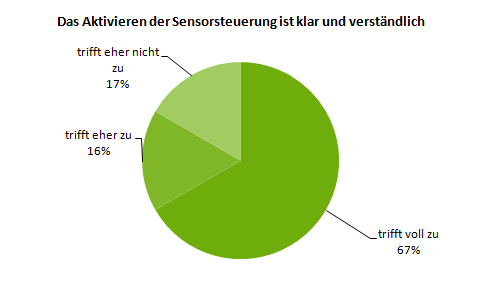
\includegraphics[width=0.85\textwidth]{03_Grafiken/Anhang/UsabilityDiagramme/Aufgabenteil4Aussage1.png}
	\caption[Diagramm zum Analysieren der Benutzerfreundlichkeit bei der Sensorsteuerung - Aussage 1]{Diagramm zum Analysieren der Benutzerfreundlichkeit bei der Sensorsteuerung - Aussage 1}
	\label{fig:Aufgabenteil4Aussage1}
\end{figure}
% ------------------------------
% Aufgabenteil 4 - Aussage 2
% ------------------------------
\begin{figure}[H]
	\centering
		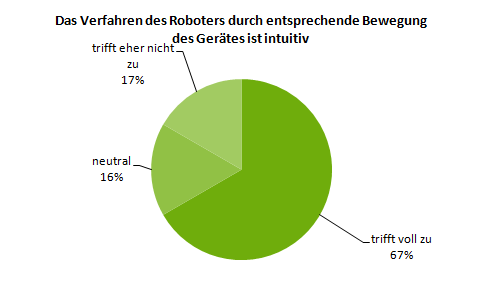
\includegraphics[width=0.85\textwidth]{03_Grafiken/Anhang/UsabilityDiagramme/Aufgabenteil4Aussage2.png}
	\caption[Diagramm zum Analysieren der Benutzerfreundlichkeit bei der Sensorsteuerung - Aussage 1]{Diagramm zum Analysieren der Benutzerfreundlichkeit bei der Sensorsteuerung - Aussage 2}
	\label{fig:Aufgabenteil4Aussage2}
\end{figure}
% ------------------------------
% Aufgabenteil 4 - Aussage 2
% ------------------------------
\begin{figure}[H]
	\centering
		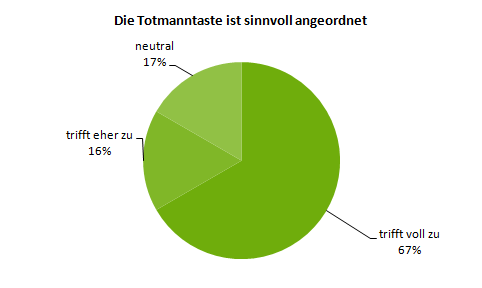
\includegraphics[width=0.85\textwidth]{03_Grafiken/Anhang/UsabilityDiagramme/Aufgabenteil4Aussage4.png}
	\caption[Diagramm zum Analysieren der Benutzerfreundlichkeit bei der Sensorsteuerung - Aussage 4]{Diagramm zum Analysieren der Benutzerfreundlichkeit bei der Sensorsteuerung - Aussage 4}
	\label{fig:Aufgabenteil4Aussage4}
\end{figure}
% ------------------------------
% Aufgabenteil 5 - Aussage 2
% ------------------------------
\begin{figure}[H]
	\centering
		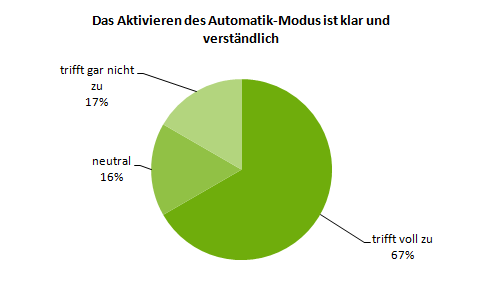
\includegraphics[width=0.85\textwidth]{03_Grafiken/Anhang/UsabilityDiagramme/Aufgabenteil5Aussage1.png}
	\caption[Diagramm zum Analysieren der Benutzerfreundlichkeit im Automatik-Modus - Aussage 1]{Diagramm zum Analysieren der Benutzerfreundlichkeit im Automatik-Modus - Aussage 1}
	\label{fig:Aufgabenteil5Aussage1}
\end{figure}
% ------------------------------
% Aufgabenteil 5 - Aussage 2
% ------------------------------
\begin{figure}[H]
	\centering
		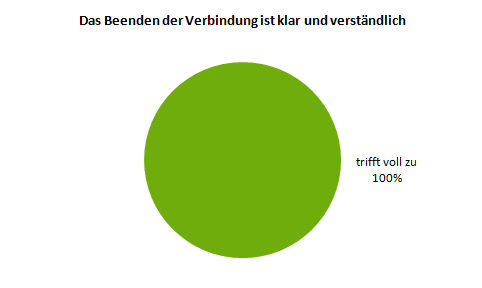
\includegraphics[width=0.85\textwidth]{03_Grafiken/Anhang/UsabilityDiagramme/Aufgabenteil5Aussage2.png}
	\caption[Diagramm zum Analysieren der Benutzerfreundlichkeit im Automatik-Modus - Aussage 2]{Diagramm zum Analysieren der Benutzerfreundlichkeit im Automatik-Modus - Aussage 2}
	\label{fig:Aufgabenteil5Aussage2}
\end{figure}
%
% Klassendiagramme
%
\newpage
%\section{Klassendiagramme}
\label{app:Klassendiagramme}
\subsection{Name Klasse 1}
%
% Bild der Klasse NAME
%
\begin{figure}[H]
\centering

\includegraphics[width=0.7\linewidth]{03_Grafiken/Anhang/Klassendiagramme/pseudoImage}
\caption[Klasse NAME]{Klasse NAME}
\label{fig:pseudoimage}
\end{figure}


%
% Details der Klasse NAME
%
\begin{center}
\renewcommand{\arraystretch}{1.2} 
\newcolumntype{C}[1]{>{\centering\arraybackslash}p{#1}}
\centering
\begin{longtable}{|p{2cm}p{12cm}|}
\caption{Parameter der Klasse NAME}\label{tab:KlasseParameter-NAME}\\
\hline 
\multicolumn{2}{|l|}{\cellcolor{gray}\textbf{Attribute}} \\ 
\hline 
\multicolumn{2}{|l|}{Element-Name + Datentyp (z.B. Button)}\\
 & Beschreibung der Funktion \\ 
\hline 
\multicolumn{2}{|l|}{Element-Name + Datentyp (z.B. Button)} \\
\multicolumn{2}{|l|}{Weitere Element-Namen + Datentyp (z.B. Button)} \\
& Beschreibung der Funktion \\ 
\hline 
%
% METHODEN
%
\multicolumn{2}{|l|}{\cellcolor{gray}\textbf{Methoden}} \\ 
\hline 
\multicolumn{2}{|l|}{Funktion-Name (z.B. protected void NAME())} \\ 
& Beschreibung der Funktion  \\
\hline 
\multicolumn{2}{|l|}{Funktion-Name (z.B. protected void NAME())} \\
& Beschreibung der Funktion \\ 
\hline 
%
% SCHNITTSTELLEN
%
\multicolumn{2}{|l|}{\cellcolor{gray}\textbf{Schnittstellen}} \\ 
\hline 
\multicolumn{2}{|l|}{Schnittstellen-Name (z.B. public interface NAME())} \\ 
\multicolumn{2}{|l|}{Funktion-Name (z.B. public void NAME())} \\ 
& Beschreibung der Schnittstelle  \\
\hline 
\end{longtable} 
\end{center}
\newpage
\subsection{Name Klasse 2}
%
% Bild der Klasse NAME
%
\begin{figure}[H]
	\centering
	
\includegraphics[width=0.7\linewidth]{03_Grafiken/pseudoImage}
	\caption[Klasse NAME]{Klasse NAME}
	\label{fig:pseudoimage}
\end{figure}

%
% Details der Klasse NAME
%
\begin{center}
	\renewcommand{\arraystretch}{1.2} 
	\newcolumntype{C}[1]{>{\centering\arraybackslash}p{#1}}
	\centering
	\begin{longtable}{|p{2cm}p{12cm}|}
		\caption{Parameter der Klasse NAME}\label{tab:KlasseParameter-NAME}\\
		\hline 
		\multicolumn{2}{|l|}{\cellcolor{gray}\textbf{Attribute}} \\ 
		\hline 
		\multicolumn{2}{|l|}{Element-Name + Datentyp (z.B. Button)}\\
		& Beschreibung der Funktion \\ 
		\hline 
		\multicolumn{2}{|l|}{Element-Name + Datentyp (z.B. Button)} \\
		\multicolumn{2}{|l|}{Weitere Element-Namen + Datentyp (z.B. Button)} \\
		& Beschreibung der Funktion \\ 
		\hline 
		%
		% METHODEN
		%
		\multicolumn{2}{|l|}{\cellcolor{gray}\textbf{Methoden}} \\ 
		\hline 
		\multicolumn{2}{|l|}{Funktion-Name (z.B. protected void NAME())} \\ 
		& Beschreibung der Funktion  \\
		\hline 
		\multicolumn{2}{|l|}{Funktion-Name (z.B. protected void NAME())} \\
		& Beschreibung der Funktion \\ 
		\hline 
		%
		% SCHNITTSTELLEN
		%
		\multicolumn{2}{|l|}{\cellcolor{gray}\textbf{Schnittstellen}} \\ 
		\hline 
		\multicolumn{2}{|l|}{Schnittstellen-Name (z.B. public interface NAME())} \\ 
		\multicolumn{2}{|l|}{Funktion-Name (z.B. public void NAME())} \\ 
		& Beschreibung der Schnittstelle  \\
		\hline 
	\end{longtable} 
\end{center}
%
% Ablauf der Anwendungsfalldiagramme
%
%\section{Ablauf der Anwendungsfalldiagramme}
\label{app:UseCasesAblauf}
\begin{table}[H]
\caption{Ablauf: NAME}\label{app:UseCaseNAME2}
\renewcommand{\arraystretch}{1.5} 
\newcolumntype{C}[1]{>{\centering\arraybackslash}p{#1}}
\centering
\begin{tabular}{|p{1.5cm}|p{1.5cm}|p{9cm}|}
 	\hline 
    \multicolumn{2}{|l|}{\cellcolor{hellgrau}\textbf{Name}} & Manuelles Verfahren des Roboters \\     
    \hline
    \multicolumn{2}{|l|}{\cellcolor{hellgrau}\textbf{Ziel}} & Verfahren des Roboters mit Tasten \\
    \hline
    \multicolumn{2}{|l|}{\cellcolor{hellgrau}\textbf{Akteure}} & Bediener, Roboter \\   
    \hline
    \multicolumn{2}{|l|}{\cellcolor{hellgrau}\textbf{Trigger}} & Starten des Steuerungsmen�s durch Bet�tigen der Verbindungstaste  \\   
    \hline
    \multicolumn{2}{|l|}{\cellcolor{hellgrau}\textbf{Vorbedingung}} & Aktive Datenverbindung zum Roboter \\   
    \specialrule{2pt}{0pt}{0pt} 
    \rowcolor{hellgrau} \textbf{Schritt} & \textbf{Akteur} & \textbf{Ablauf} \\
    \hline
    1. & Person & Aktivieren des manuellen Betriebsmodus \\
    \hline
    2. & Person & Einstellen der gew�nschten Geschwindigkeit \\
    \hline
    3. & Person & Verfahren des Roboters in die gew�nschte Ausgangsorientierung \\
    \hline
    4. & Roboter & Abarbeiten der empfangenen Beschleunigungswerte \\
    \hline
\end{tabular} 
\end{table}
\begin{table}[H]
\caption{Ablauf: NAME}\label{app:UseCaseNAME1}
\renewcommand{\arraystretch}{1.5} 
\newcolumntype{C}[1]{>{\centering\arraybackslash}p{#1}}
\centering
\begin{tabular}{|p{1.5cm}|p{1.5cm}|p{9cm}|}
 	\hline 
    \multicolumn{2}{|l|}{\cellcolor{hellgrau}\textbf{Name}} & Verbindung einrichten \\     
    \hline
    \multicolumn{2}{|l|}{\cellcolor{hellgrau}\textbf{Ziel}} & Verbindung zum Roboter aufbauen \\
    \hline
    \multicolumn{2}{|l|}{\cellcolor{hellgrau}\textbf{Akteure}} & Bediener \\   
    \hline
    \multicolumn{2}{|l|}{\cellcolor{hellgrau}\textbf{Trigger}} & Starten der Anwendung FloriBot HMI \\   
    \hline
    \multicolumn{2}{|l|}{\cellcolor{hellgrau}\textbf{Vorbedingung}} & Flugmodus ist aktiv \\   
    \specialrule{2pt}{0pt}{0pt} 
    \rowcolor{hellgrau} \textbf{Schritt} & \textbf{Akteur} & \textbf{Ablauf} \\
    \hline
    1. & Person & Eingabe der Master-Adresse \\
    \hline
    2. & Person & Eingabe des Publisher-Topics \\
    \hline
    3. & Person & Eingabe des Subscriber-Topics \\
    \hline
    4. & Person & Eingabe des Node Namens im Optionsmen� \\
    \hline
    5. & Person & Setzen des Themes im Optionsmen� \\
    \hline
    6. & Person & Bet�tigen der Verbindungstaste zum Starten des Verbindungsaufbaus \\
	\hline 
	\rowcolor{hellgrau} & & \textbf{Erweiterung} \\
	7.a &  & Kein Verbindungsaufbau m�glich, wenn Flugmodus deaktiviert. Ein Hinweis wird ausgegeben. \\
    \hline
    7.b &  & Kein Verbindungsaufbau m�glich, wenn nicht alle Eingabefelder ausgef�llt sind. Ein Hinweis wird ausgegeben. \\
    \hline
    7.c &  & Kein Verbindungsaufbau m�glich, wenn Wlan-Schnittstelle deaktiviert ist. Ein Hinweis wird ausgegeben. \\
	\hline 
\end{tabular} 
\end{table}
%
% Listings
%
\section{Listings}
\label{app:Quellcode}
\subsection{Listing 1}
\label{app:Listing1}
\begin{lstlisting}[language=Java, caption=NAME]
public void Function {

}
\end{lstlisting}
%
% --------------------------------------------
%
\begin{lstlisting}[language=Java, caption=NAME]
public void Function {

}
\end{lstlisting}
\newpage
\subsection{Listing 2}
\label{app:Listing2}
\begin{lstlisting}[language=Java, caption=NAME]
public void Function {

}
\end{lstlisting}
%
% --------------------------------------------
%
\begin{lstlisting}[language=Java, caption=NAME]
public void Function {

}
\end{lstlisting}
%
% Fehlermeldungen und Bugs
%
%\section{Fehlermeldungen und Bugs}
\label{FehlerBugs}
In der folgend dargestellten Tabelle sind die derzeit vorhandenen Bugs der Software \textit{NAME} aufgelistet. Dabei wird, neben einer Beschreibung des Fehlers, der Kontext genannt, in dem das Auftreten erfolgt und ein Indikator aufgezeigt, der die Bedeutung des Fehlers wiedergibt.\\
Die Farben des Indikators sind definiert mit:
\begin{table}[H]
\centering
\begin{tabular}{ll}
\textcolor{red}{Rot:} & Stark \\ 
\textcolor{yellow}{Gelb:} & Mittel \\ 
\textcolor{green}{Gr�n:} & Schwach \\ 
\end{tabular} 
\end{table}

\begin{table}[H]
\caption{Liste von bekannten Bugs der Software NAME HMI}\label{app:BugListe}
\renewcommand{\arraystretch}{1.5} 
\newcolumntype{C}[1]{>{\centering\arraybackslash}p{#1}}
\centering
\begin{tabular}{|p{4.5cm}|p{3cm}|C{6cm}|}
 	\hline 
    \rowcolor{hellgrau} \textbf{Fehlerbeschreibung} & \textbf{Kontext} & \textbf{Sicherheitsbeeintr�chtigung}\\
    \hline
    Fehlerbeschreibung & Kontext & \redDot{-0.4} \\
    \hline
    Fehlerbeschreibung & Kontext & \redDot{-1.3} \\
    \hline
    Fehlerbeschreibung & Kontext & \greenDot{-0.6} \\
    \hline
    Fehlerbeschreibung & Kontext & \yellowDot{-1.2} \\
    \hline
    Fehlerbeschreibung & Kontext & \greenDot{-1.2} \\
    \hline
    Fehlerbeschreibung & Kontext & \greenDot{-1.2} \\
    \hline
\end{tabular} 
\end{table}

\newpage
Folgende Tabelle zeigt eine �bersicht der Fehlermeldungen, durch die der Bediener der Software \gls{NAME} �ber m�gliche fehlerhafte Eingaben und nicht unterst�tzte Handhabung informiert wird. Dabei ist, neben der Beschreibung der Fehlermeldung, der Kontext, indem der Fehler auftritt und der L�sungsvorschlag genannt.
\begin{table}[htb]
\caption{Fehlermeldungen der Software NAME}\label{app:Fehlermeldungen}
\renewcommand{\arraystretch}{1.5} 
\newcolumntype{C}[1]{>{\centering\arraybackslash}p{#1}}
\centering
\begin{tabular}{|p{4.5cm}|p{4.5cm}|p{4.5cm}|}
 	\hline 
    \rowcolor{hellgrau} \textbf{Fehlermeldung} & \textbf{Kontext} & \textbf{L�sung} \\
    \hline
    Fehlermeldung & Kontext & L�sung \\
    \hline
    Fehlermeldung & Kontext & L�sung \\
    \hline
    Fehlermeldung & Kontext & L�sung\\
    \hline
    Fehlermeldung & Kontext & L�sung\\
    \hline
    Fehlermeldung & Kontext & L�sung\\
    \hline
    Fehlermeldung & Kontext & L�sung\\
    \hline
    Fehlermeldung & Kontext & L�sung\\
    \hline
    Fehlermeldung & Kontext & L�sung\\
    \hline
    Fehlermeldung & Kontext & L�sung
\end{tabular} 
\end{table}
%
% Erklaerung
%
\postappendix
\listoffigures
\listoftables
\printglossary[type=\acronymtype]%, style=listdotted
\printglossary
%\addchap{Verzeichnis Daten-CD}
%Dieses Verzeichnis zeigt die wichtigsten Bestandteile der Daten-CD. Dabei stellt das Zeichen + einen Ordner und das Zeichen - eine Datei dar.

\vspace{1cm}
\parbox{0cm}{\begin{tabbing}
x \= x \= x \= x \= x \= x \kill
- Datei1 \\
- Datei2 \\
+ Ordner1 \\
+ Ordner2 \\
\> + Unterordner1-Ebene1 \\
\>\> + Unterordner1-Ebene2 \\
\>\>\> + Unterordner1-Ebene3 \\
\>\>\>\> + Unterordner1-Ebene4 \\
\>\>\>\> + Unterordner2-Ebene4 \\
\>\>\>\> + ... \\
\>\> + Unterordner2-Ebene2 \\
\>\>\> - Datei \\
\>\> + Unterordner3-Ebene2 \\
\>\>\> + Unterordner2-Ebene3 \\
\>\>\> + Unterordner3-Ebene3 \\
\>\>\> + ... \\
+ Ordner3 \\
\> + Unterordner2-Ebene1 \\
\>\> + Unterordner4-Ebene2 \\
\>\>\> + Unterordner1-Ebene4 \\
\end{tabbing}}
\addchap{Erkl�rung} 
\refstepcounter{chapter}
%\section{Erkl�rung}
Hiermit erkl�re ich an Eides Statt, dass ich die vorliegende Arbeit selbst�ndig und ohne 
Benutzung anderer als der angegebenen Hilfsmittel angefertigt habe. Die aus fremden 
Quellen direkt oder indirekt �bernommenen Gedanken sind als solche kenntlich gemacht. 

ORT, {DATUM}
%\\[30pt]
\vspace{-0.2cm}
\begin{figure}[H]
	
\includegraphics[width=0.25\textwidth]{03_Grafiken/Anhang/mySignature.jpg}
\end{figure}
\vspace{-1cm}
Manuel-Leonhard Rixen

%%\section{Verwendete Symbole und Begriffe}
%%\input{99_Anhang/SymboleBegriffe}				
    
	
%%%%%%%%%%%%%%%%%%%%%%%%%%%%%%%%%%%%%%%%%%%%%%%%%%%%%%
\end{document} 
% ----------------------------------------------
